\chapter{Hiện thực hệ thống}

Chương này trình bày quá trình hiện thực các chức năng chính của hệ thống Social Commerce dựa trên các yêu cầu và thiết kế đã được phân tích ở các chương trước. Nội dung chương tập trung mô tả các giao diện đã được triển khai thực tế, luồng hoạt động của từng chức năng và cách người dùng tương tác với hệ thống.

Các chức năng được tổ chức theo từng module tương ứng với kiến trúc hệ thống, bao gồm: quản lý người dùng và xác thực, tương tác xã hội, hoạt động thương mại, hệ thống quản trị, hỗ trợ tạo nội dung bằng AI, quản lý bài đăng đã lên lịch và hệ thống thông báo thời gian thực.

Toàn bộ giao diện minh họa trong chương này đều là giao diện thực tế của hệ thống đã được hiện thực và kiểm thử trong quá trình phát triển dự án.

\section{Module 1: Quản lý Người dùng và Xác thực}

Module này bao gồm các giao diện liên quan đến việc đăng ký, đăng nhập, quản lý tài khoản và cài đặt người dùng.

\subsection{Trang Đăng ký}

Trang đăng ký cho phép người dùng tạo tài khoản mới để sử dụng đầy đủ các chức năng của hệ thống Social Commerce. Người dùng cần cung cấp các thông tin cơ bản bao gồm email, mật khẩu và xác nhận mật khẩu để hoàn tất quá trình đăng ký tài khoản.

Hệ thống thực hiện kiểm tra tính hợp lệ của dữ liệu đầu vào như định dạng email, độ mạnh mật khẩu và sự khớp nhau giữa mật khẩu xác nhận và mật khẩu chính nhằm đảm bảo tính chính xác và an toàn cho thông tin người dùng. Sau khi đăng ký thành công, dữ liệu tài khoản sẽ được lưu trữ vào cơ sở dữ liệu và người dùng có thể đăng nhập để sử dụng các chức năng cá nhân hóa của hệ thống.

Giao diện được thiết kế theo hướng tối giản và trực quan nhằm giúp người dùng thao tác dễ dàng trên nhiều kích thước màn hình khác nhau.

\begin{figure}[H]
\centering
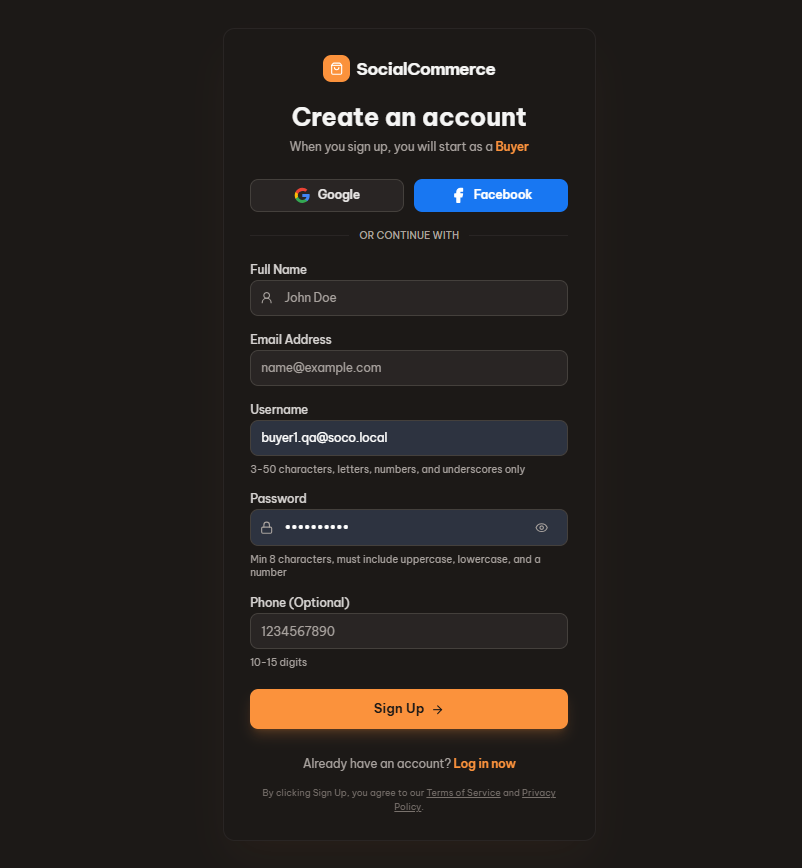
\includegraphics[width=\textwidth]{Images/UI/module1/register-page.png}
\caption{Giao diện đăng ký tài khoản}
\label{fig}
\end{figure}

\subsection{Trang Đăng nhập}

Trang đăng nhập cho phép người dùng truy cập vào hệ thống bằng tài khoản đã đăng ký trước đó. Người dùng có thể đăng nhập thông qua email hoặc tên đăng nhập kết hợp với mật khẩu tương ứng. Giao diện cũng hỗ trợ các chức năng như ghi nhớ đăng nhập và khôi phục mật khẩu trong trường hợp người dùng quên thông tin tài khoản.

Để tăng cường tính bảo mật cho hệ thống, chức năng xác thực hai lớp (2FA) qua email được hỗ trợ đối với các tài khoản đã kích hoạt tính năng này. Sau khi người dùng nhập đúng thông tin đăng nhập, hệ thống sẽ gửi mã OTP gồm 6 chữ số đến địa chỉ email đã đăng ký. Người dùng cần nhập chính xác mã OTP để hoàn tất quá trình xác thực và truy cập vào hệ thống.

Giao diện xác thực 2FA hiển thị ô nhập mã OTP, bộ đếm thời gian hiệu lực của mã và chức năng gửi lại mã xác thực khi cần thiết. Cơ chế này giúp hạn chế các truy cập trái phép và nâng cao độ an toàn cho tài khoản người dùng.

\begin{figure}[H]
\centering
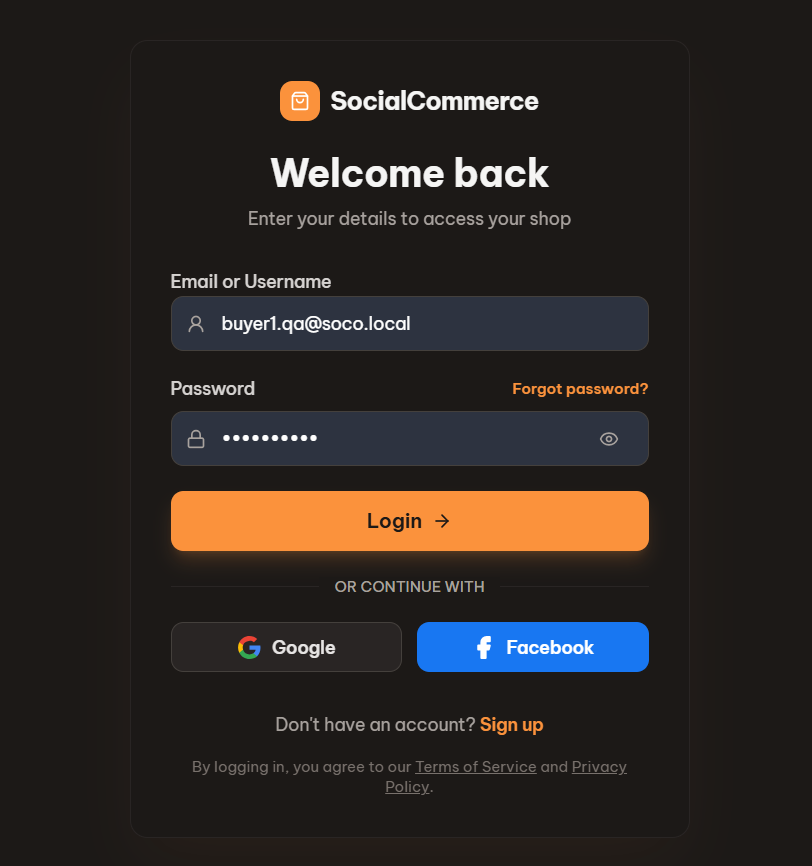
\includegraphics[width=\textwidth]{Images/UI/module1/login-page.png}
\caption{Giao diện đăng nhập của hệ thống}
\label{fig}
\end{figure}

\begin{figure}[H]
\centering
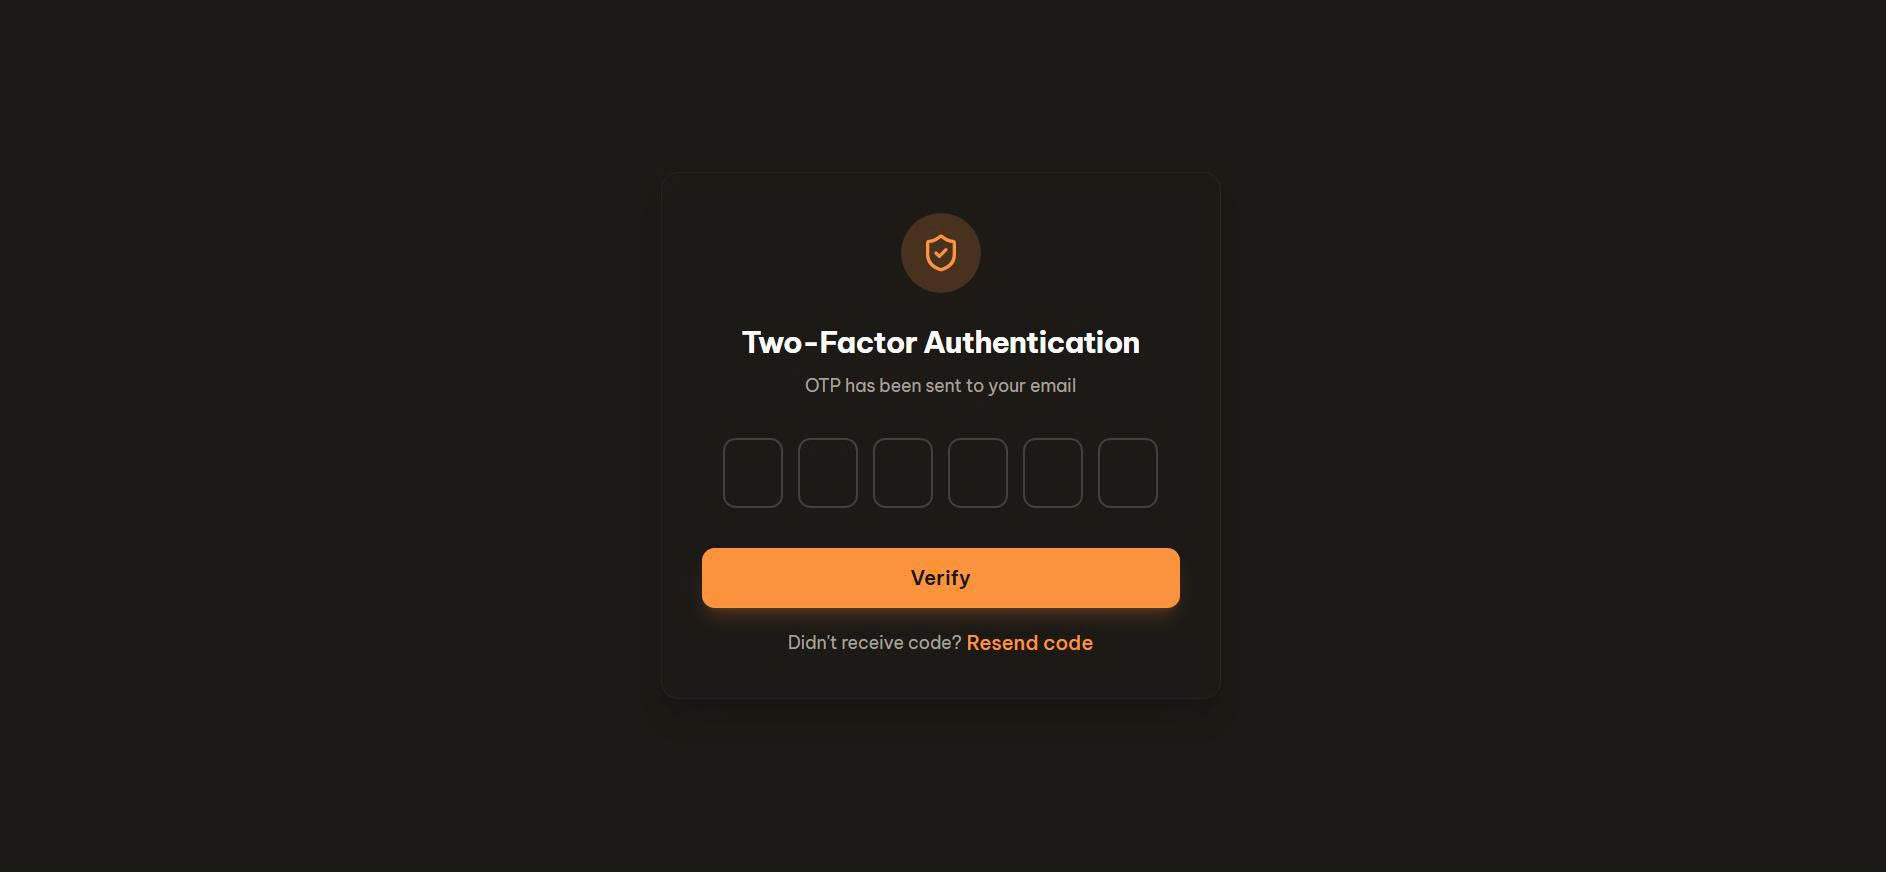
\includegraphics[width=\textwidth]{Images/UI/module1/two-factor-authentication.png}
\caption{Giao diện xác thực hai lớp (2FA)}
\label{fig}
\end{figure}

\subsection{Trang Quên mật khẩu}
Trang quên mật khẩu hỗ trợ người dùng khôi phục lại tài khoản trong trường hợp không thể đăng nhập do quên mật khẩu. Quy trình khôi phục được thực hiện thông qua email nhằm đảm bảo tính bảo mật và xác thực đúng chủ sở hữu tài khoản.

Người dùng cần nhập địa chỉ email đã đăng ký để nhận mã OTP xác thực từ hệ thống. Sau khi nhập đúng mã OTP còn hiệu lực, người dùng có thể thiết lập mật khẩu mới để tiếp tục sử dụng tài khoản. Hệ thống đồng thời kiểm tra tính hợp lệ và độ an toàn của mật khẩu mới trước khi cập nhật vào cơ sở dữ liệu.

Giao diện được xây dựng theo quy trình từng bước nhằm giúp người dùng dễ dàng thao tác và hạn chế các lỗi trong quá trình khôi phục mật khẩu.

\begin{figure}[H]
\centering
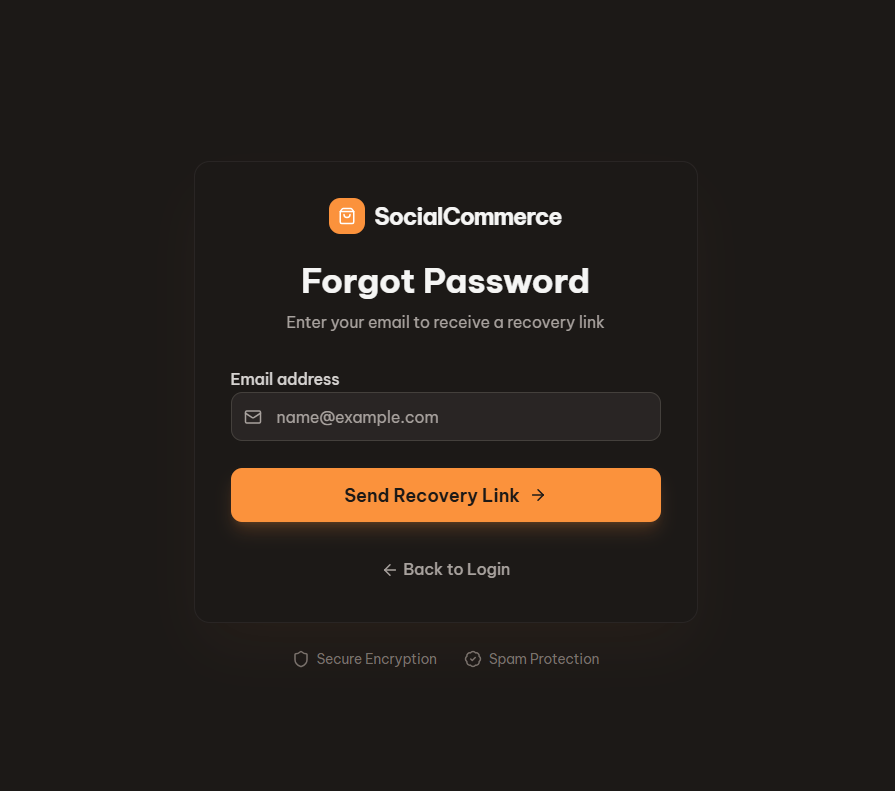
\includegraphics[width=\textwidth]{Images/UI/module1/forgot-password-page.png}
\caption{Giao diện khôi phục mật khẩu}
\label{fig}
\end{figure}

\subsection{Trang Hồ sơ cá nhân}

Trang hồ sơ cá nhân cho phép người dùng quản lý và hiển thị các thông tin liên quan đến tài khoản của mình trên hệ thống Social Commerce. Giao diện hồ sơ được phân chia thành hai loại tùy theo vai trò của người dùng bao gồm hồ sơ người mua và hồ sơ người bán.

\textbf{Hồ sơ Người mua (Buyer Profile):} Giao diện hiển thị các thông tin cơ bản của người dùng như ảnh đại diện, ảnh bìa, tên hiển thị, mô tả cá nhân, số lượng người theo dõi, số lượng đang theo dõi và danh sách các bài đăng đã chia sẻ trên hệ thống. Người dùng có thể chỉnh sửa thông tin cá nhân trực tiếp thông qua giao diện hồ sơ nhằm cá nhân hóa trải nghiệm sử dụng.

\textbf{Hồ sơ Người bán (Seller Profile):} Ngoài các thông tin cơ bản tương tự hồ sơ người mua, hồ sơ người bán còn hiển thị thêm danh sách sản phẩm đang kinh doanh, thông tin đánh giá từ khách hàng và các chỉ số liên quan đến hoạt động bán hàng. Các đánh giá và nhận xét từ người mua giúp tăng độ tin cậy cho cửa hàng và hỗ trợ người dùng khác trong quá trình tham khảo sản phẩm trước khi mua hàng.

Giao diện hồ sơ được xây dựng theo hướng trực quan và tối ưu trải nghiệm người dùng, đồng thời hỗ trợ hiển thị tốt trên nhiều loại thiết bị khác nhau.

\begin{figure}[H]
\centering
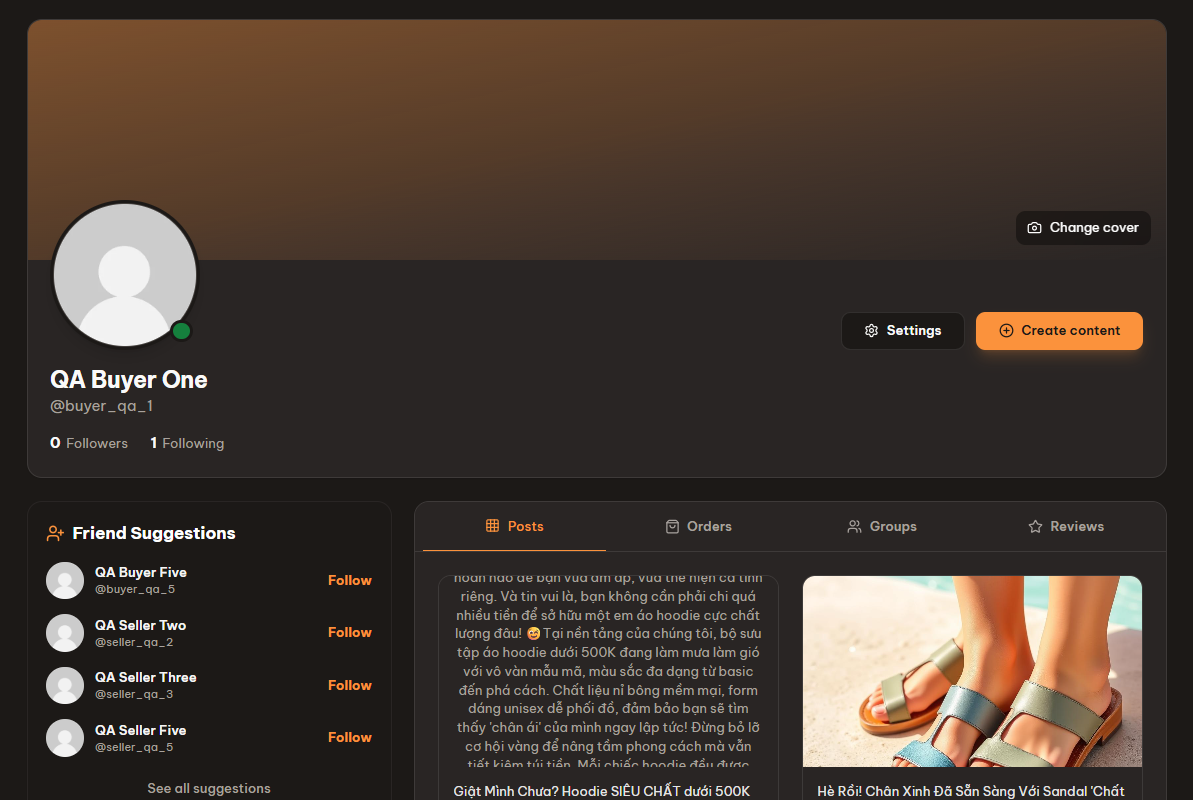
\includegraphics[width=\textwidth]{Images/UI/module1/buyer-profile.png}
\caption{Giao diện hồ sơ người mua}
\label{fig}
\end{figure}

\begin{figure}[H]
\centering
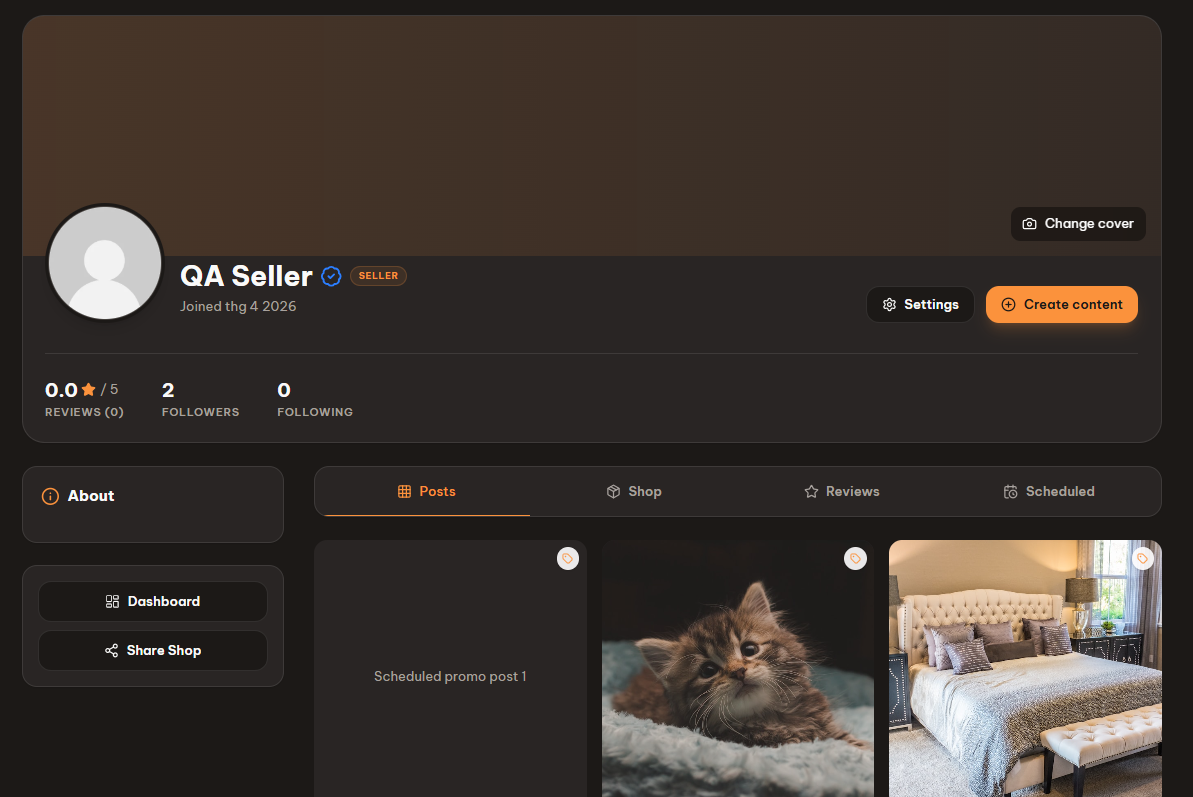
\includegraphics[width=\textwidth]{Images/UI/module1/seller-profile.png}
\caption{Giao diện hồ sơ người bán}
\label{fig}
\end{figure}

\subsection{Trang Cài đặt}

Trang cài đặt cho phép người dùng quản lý các thông tin và tùy chọn liên quan đến tài khoản cá nhân. Giao diện được tổ chức theo từng nhóm chức năng nhằm giúp người dùng dễ dàng thao tác và quản lý thông tin trên hệ thống.

Người dùng có thể cập nhật thông tin cá nhân, thay đổi mật khẩu, cấu hình quyền riêng tư và quản lý các tùy chọn thông báo. Các thay đổi sẽ được kiểm tra tính hợp lệ trước khi cập nhật vào cơ sở dữ liệu nhằm đảm bảo tính chính xác và an toàn cho dữ liệu người dùng.

\begin{figure}[H]
\centering
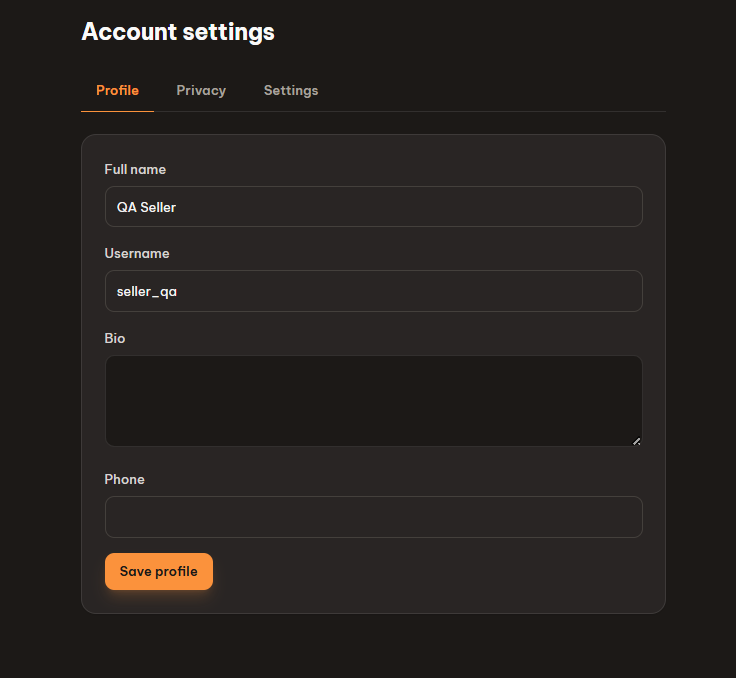
\includegraphics[width=\textwidth]{Images/UI/module1/settings-page.png}
\caption{Giao diện cài đặt tài khoản}
\label{fig}
\end{figure}

\subsection{Trang Đăng ký Người bán}

Chức năng đăng ký người bán cho phép người dùng nâng cấp tài khoản cá nhân thành tài khoản người bán để sử dụng các chức năng thương mại trên hệ thống như quản lý sản phẩm, quản lý đơn hàng và theo dõi hoạt động kinh doanh.

Quy trình đăng ký được xây dựng theo dạng nhiều bước nhằm giúp người dùng dễ dàng cung cấp đầy đủ các thông tin cần thiết và tăng tính trực quan trong quá trình đăng ký. Hệ thống bao gồm ba bước chính: thông tin cửa hàng, xác minh danh tính và thiết lập thanh toán.

Ở bước đầu tiên, người dùng cần cung cấp các thông tin cơ bản của cửa hàng như tên cửa hàng, danh mục kinh doanh, mô tả, địa chỉ liên hệ, logo và ảnh bìa đại diện cho cửa hàng. Các hình ảnh tải lên sẽ được lưu trữ thông qua dịch vụ Cloudinary nhằm hỗ trợ quản lý và hiển thị dữ liệu hiệu quả.

\begin{figure}[H]
\centering
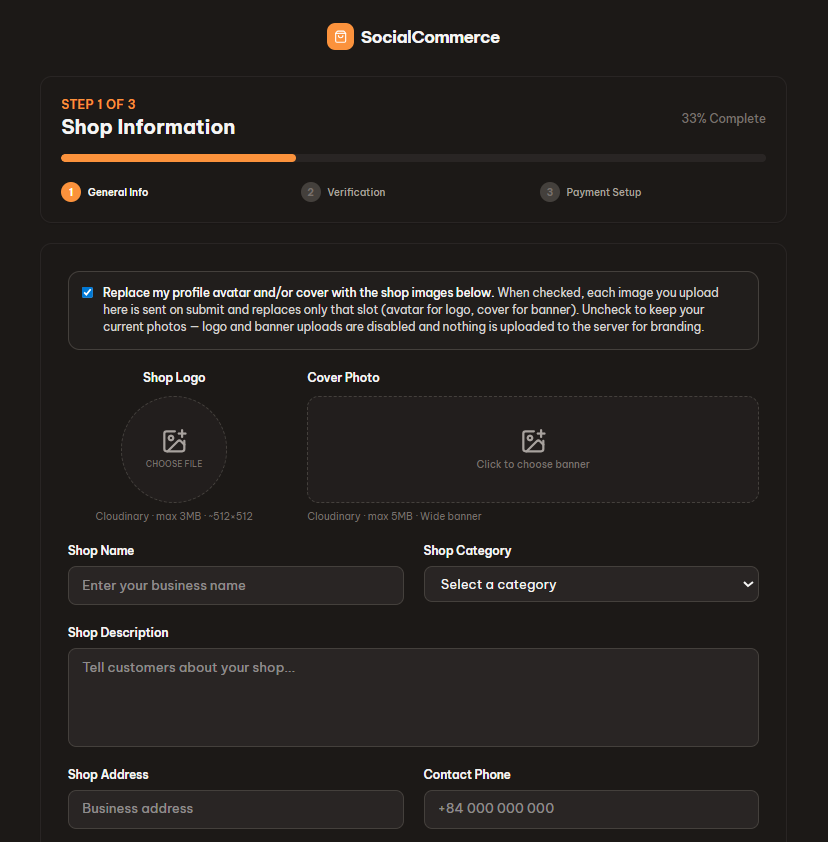
\includegraphics[width=\textwidth]{Images/UI/module1/become-seller-step1.png}
\caption{Giao diện đăng ký người bán - Bước 1: Thông tin cửa hàng}
\label{fig}
\end{figure}

Ở bước thứ hai, người dùng thực hiện xác minh danh tính bằng cách cung cấp thông tin giấy tờ xác thực như căn cước công dân, hộ chiếu hoặc giấy phép kinh doanh. Hệ thống hỗ trợ tải lên hình ảnh giấy tờ nhằm phục vụ quá trình xét duyệt và đảm bảo tính minh bạch cho tài khoản người bán.

\begin{figure}[H]
\centering
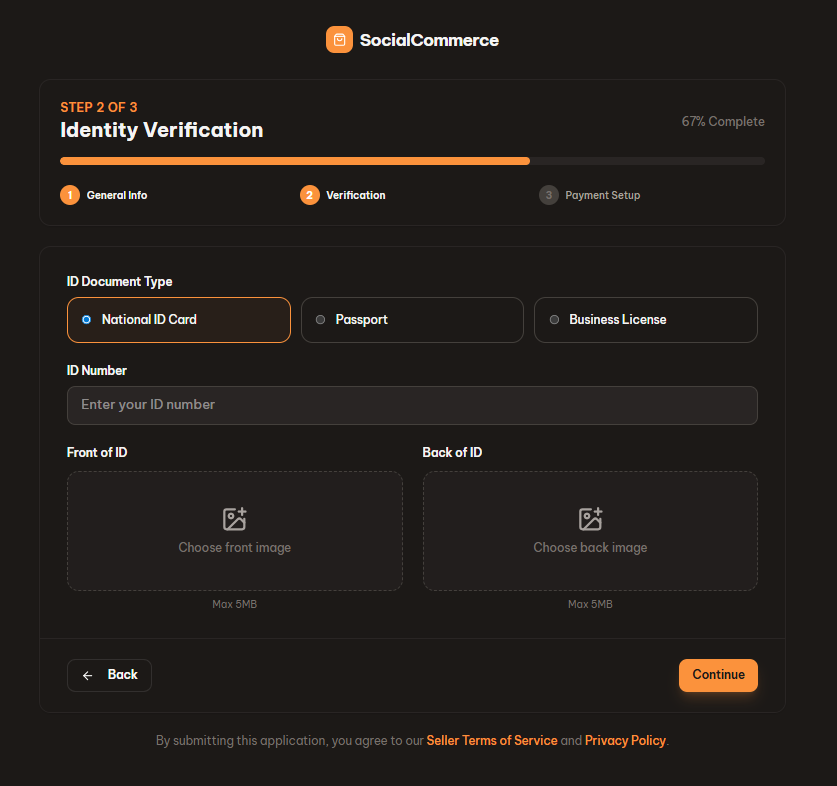
\includegraphics[width=\textwidth]{Images/UI/module1/become-seller-step2.png}
\caption{Giao diện đăng ký người bán - Bước 2: Xác minh danh tính}
\label{fig}
\end{figure}

Ở bước cuối cùng, người dùng thiết lập thông tin thanh toán bao gồm tên ngân hàng, số tài khoản và tên chủ tài khoản để phục vụ cho quá trình thanh toán và đối soát doanh thu trên hệ thống.

\begin{figure}[H]
\centering
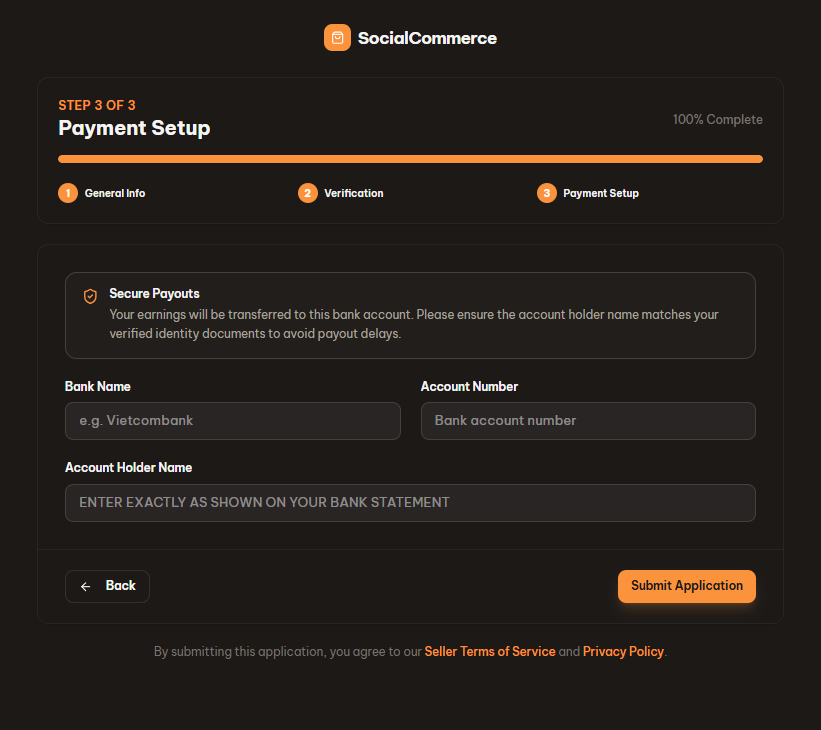
\includegraphics[width=\textwidth]{Images/UI/module1/become-seller-step3.png}
\caption{Giao diện đăng ký người bán - Bước 3: Thiết lập thanh toán}
\label{fig}
\end{figure}

Sau khi hoàn tất toàn bộ thông tin đăng ký, hệ thống sẽ gửi yêu cầu xét duyệt đến quản trị viên. Người dùng sẽ nhận được thông báo sau khi hồ sơ được gửi thành công và chờ quá trình phê duyệt từ hệ thống quản trị.

\begin{figure}[H]
\centering
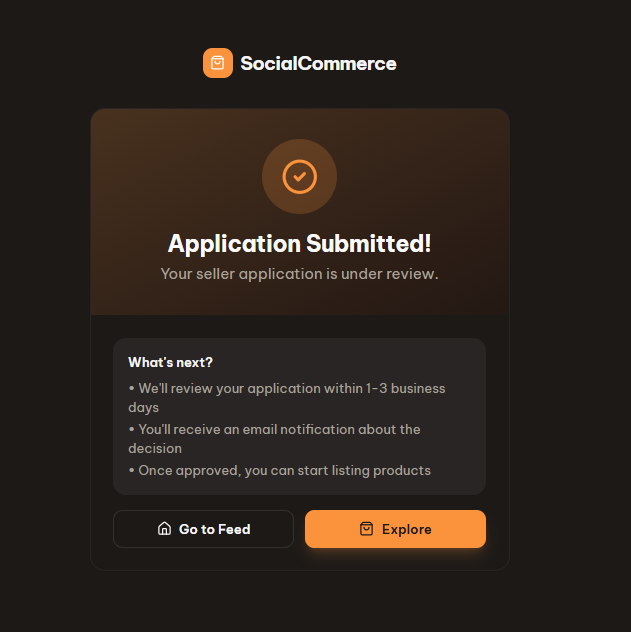
\includegraphics[width=\textwidth]{Images/UI/module1/become-seller-success.png}
\caption{Giao diện gửi đăng ký người bán thành công}
\label{fig}
\end{figure}

\section{Module 2: Tương tác Xã hội}

Module này bao gồm các chức năng hỗ trợ người dùng tương tác trên nền tảng thông qua bảng tin, tạo bài đăng, chia sẻ nội dung, bình luận và nhắn tin giữa các người dùng trong hệ thống.

\subsection{Trang chủ - Bảng tin}

Trang chủ đóng vai trò là trung tâm tương tác chính của hệ thống Social Commerce, nơi hiển thị các bài đăng mới nhất từ những người dùng và cửa hàng mà người dùng đang theo dõi. Hệ thống hỗ trợ hiển thị nội dung theo dạng bảng tin động nhằm giúp người dùng dễ dàng cập nhật các hoạt động và nội dung mới trên nền tảng.

Ngoài việc hiển thị bài đăng, giao diện còn tích hợp khu vực tạo bài viết nhanh, thanh tìm kiếm và các chức năng tương tác như thích, bình luận và chia sẻ bài đăng. Dữ liệu bảng tin được tải động và phân trang nhằm tối ưu hiệu năng hiển thị và trải nghiệm sử dụng.

\begin{figure}[H]
\centering
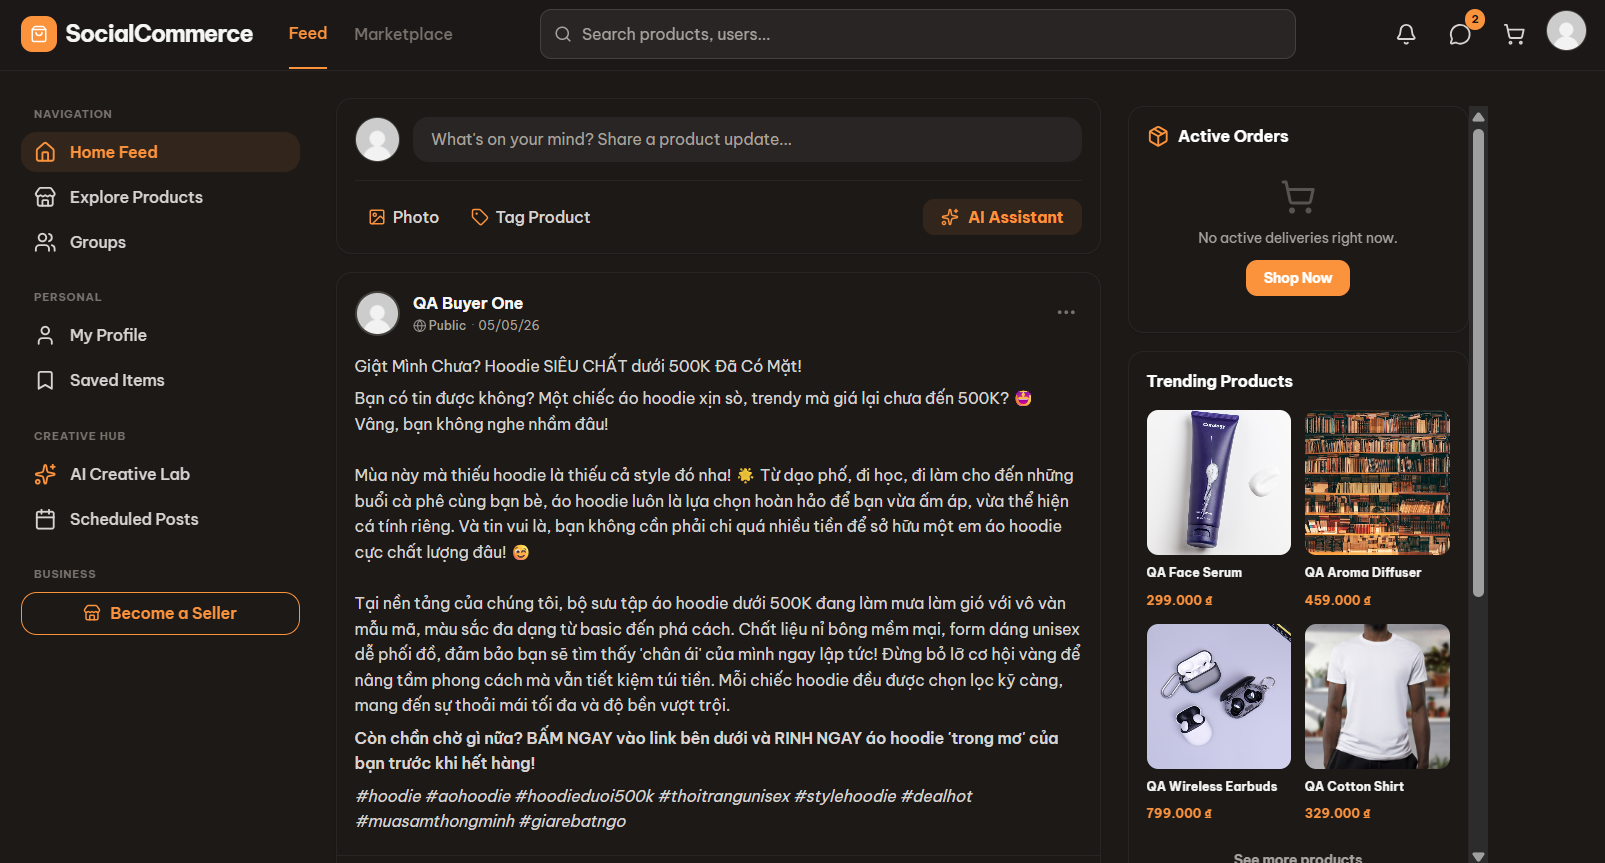
\includegraphics[width=\textwidth]{Images/UI/module2/home-feed.png}
\caption{Giao diện trang chủ - Bảng tin}
\label{fig}
\end{figure}

\subsection{Giao diện Tạo bài đăng}

Chức năng tạo bài đăng cho phép người dùng chia sẻ nội dung lên hệ thống dưới nhiều định dạng khác nhau bao gồm văn bản, hình ảnh và nội dung gắn kèm sản phẩm. Người dùng có thể nhập nội dung bài viết, tải lên hình ảnh và lựa chọn các sản phẩm liên quan để hiển thị trực tiếp trong bài đăng.

Hệ thống đồng thời hỗ trợ các tính năng mở rộng như tạo nội dung bằng AI và lên lịch đăng bài. Người dùng có thể sử dụng AI để hỗ trợ tạo nội dung văn bản, hình ảnh hoặc nội dung sáng tạo phục vụ cho hoạt động truyền thông và bán hàng trên nền tảng.

Ngoài ra, chức năng lên lịch đăng bài cho phép người dùng lựa chọn thời gian đăng tải nội dung trong tương lai. Các bài viết đã lên lịch sẽ được hệ thống tự động xử lý và đăng tải đúng thời gian đã thiết lập.

\begin{figure}[H]
\centering
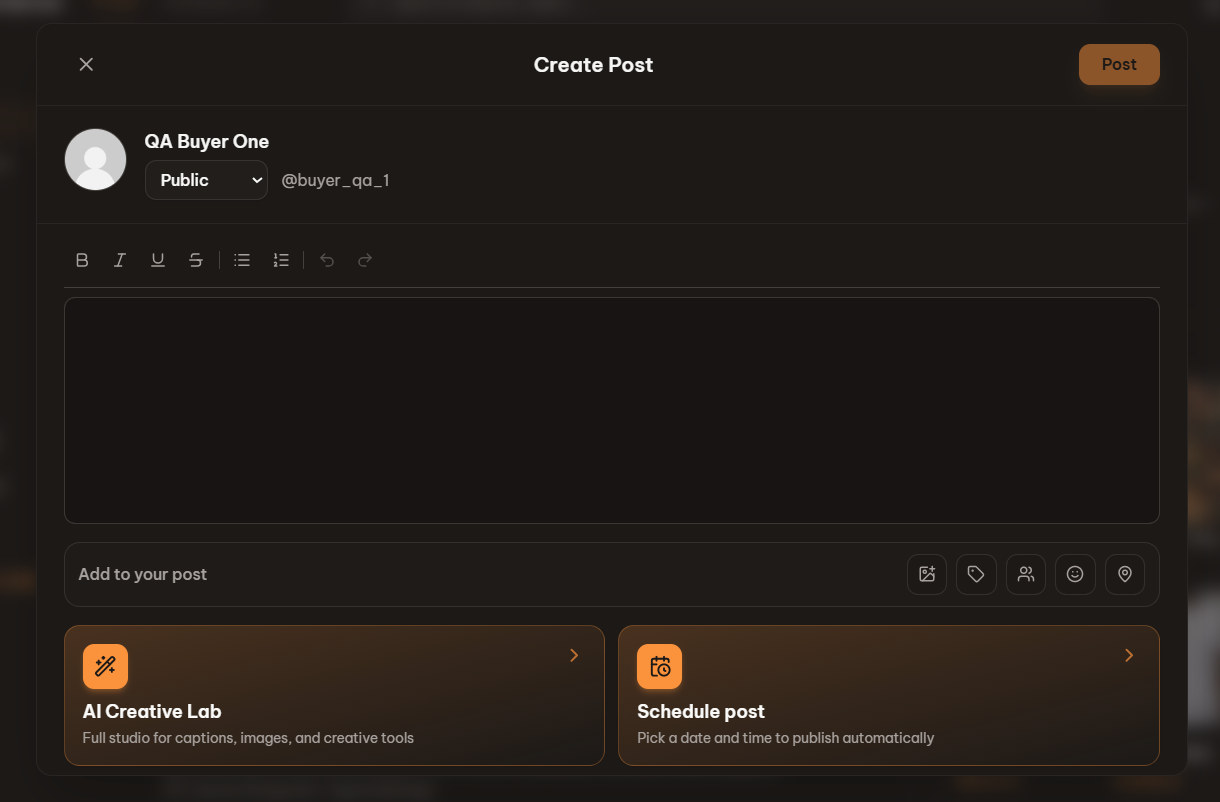
\includegraphics[width=\textwidth]{Images/UI/module2/create-post.png}
\caption{Giao diện tạo bài đăng}
\label{fig}
\end{figure}

\begin{figure}[H]
\centering
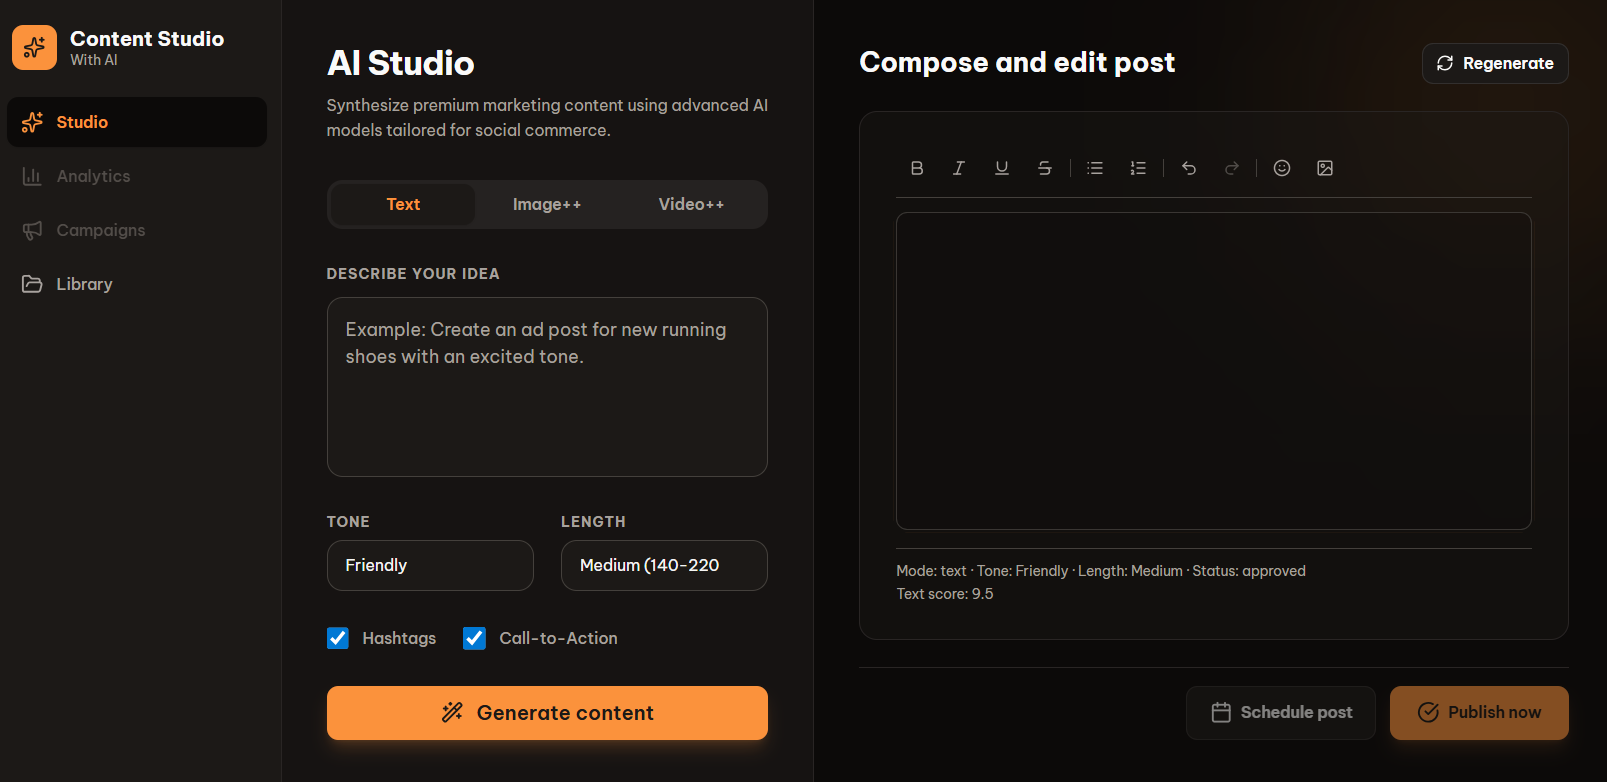
\includegraphics[width=\textwidth]{Images/UI/module2/create-post-ai-schedule.png}
\caption{Giao diện tạo bài đăng với AI và lên lịch}
\label{fig}
\end{figure}

\subsection{Trang Chi tiết Bài đăng}

Trang chi tiết bài đăng hiển thị đầy đủ nội dung của một bài viết bao gồm văn bản, hình ảnh, sản phẩm được gắn kèm và các thông tin liên quan đến người đăng bài. Người dùng có thể thực hiện các thao tác tương tác như thích bài viết, bình luận và chia sẻ nội dung trực tiếp từ giao diện này.

Hệ thống đồng thời hỗ trợ hiển thị danh sách bình luận theo thời gian thực nhằm tăng tính tương tác giữa người dùng trên nền tảng.

\begin{figure}[H]
\centering
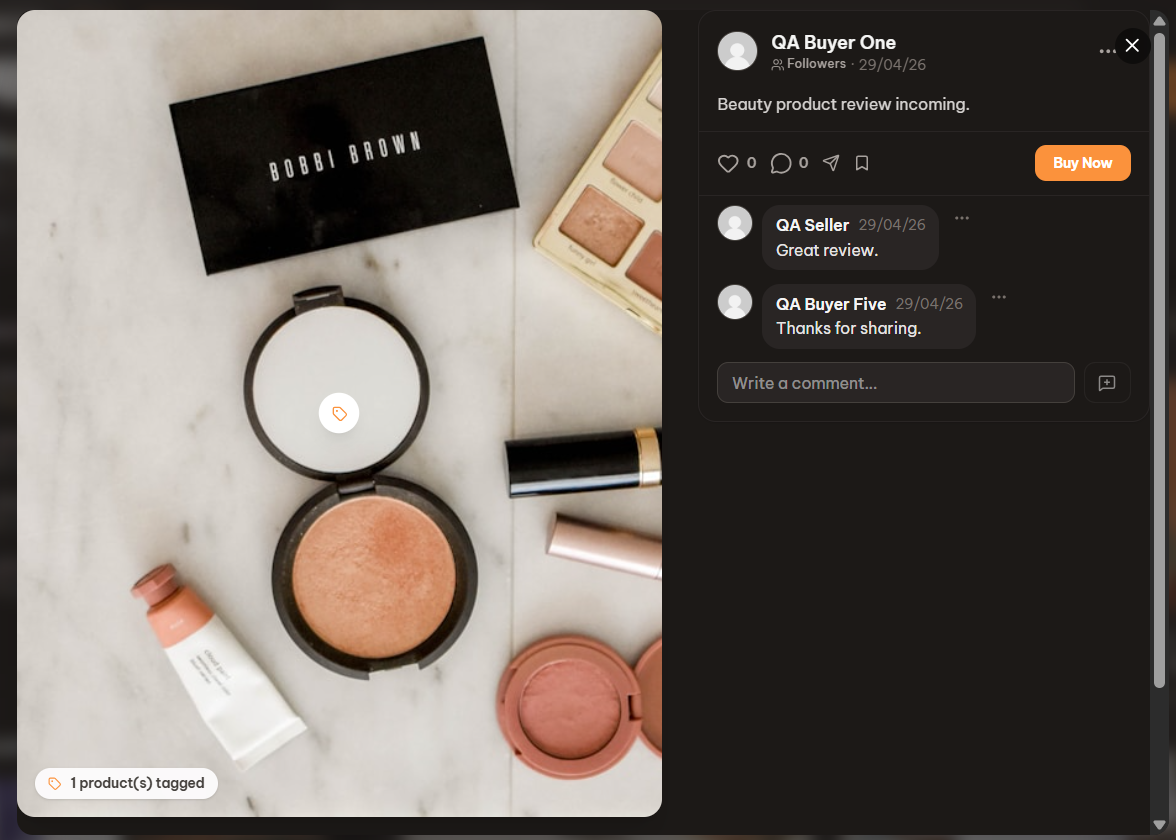
\includegraphics[width=\textwidth]{Images/UI/module2/post-detail.png}
\caption{Giao diện chi tiết bài đăng}
\label{fig}
\end{figure}

\subsection{Trang Nhắn tin}

Chức năng nhắn tin cho phép người dùng trao đổi thông tin trực tiếp với nhau ngay trên nền tảng Social Commerce. Hệ thống hỗ trợ gửi và nhận tin nhắn theo thời gian thực nhằm tăng khả năng tương tác giữa người mua và người bán trong quá trình trao đổi sản phẩm và dịch vụ.

Giao diện nhắn tin bao gồm danh sách các cuộc trò chuyện gần đây, thanh tìm kiếm và khu vực hiển thị nội dung hội thoại giữa các người dùng. Người dùng có thể theo dõi trạng thái tin nhắn chưa đọc và truy cập nhanh vào các cuộc trò chuyện trực tiếp từ giao diện hệ thống.

Hệ thống sử dụng Socket.IO để đồng bộ dữ liệu theo thời gian thực, giúp các tin nhắn mới được cập nhật trực tiếp trên giao diện mà không cần tải lại trang.

\begin{figure}[H]
\centering
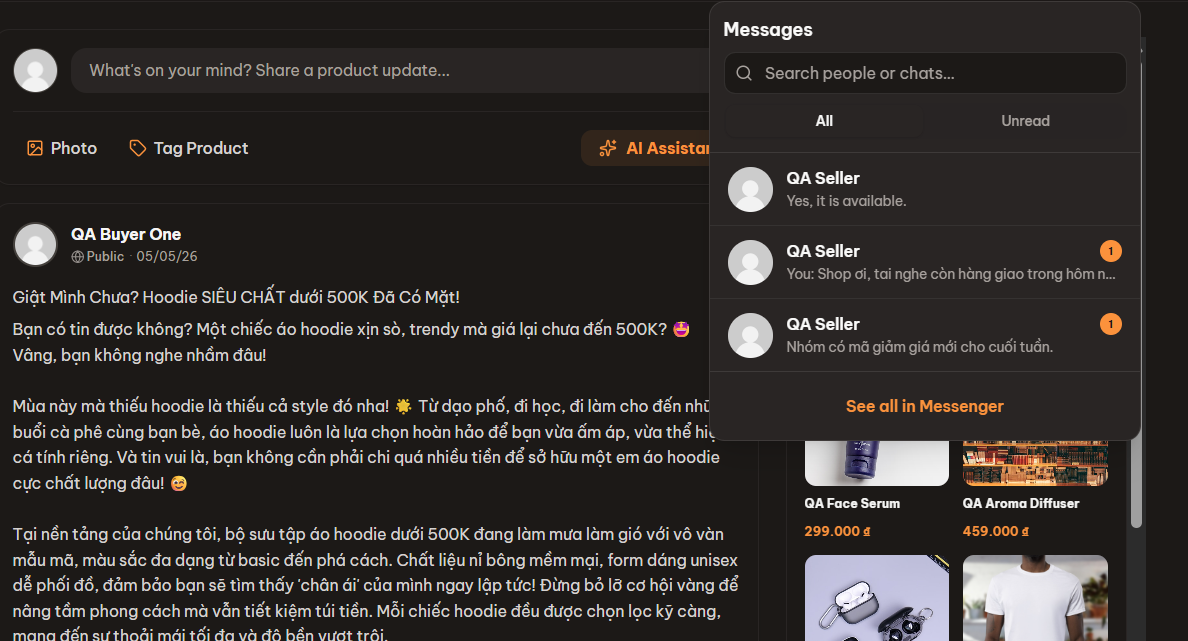
\includegraphics[width=\textwidth]{Images/UI/module2/messaging-dropdown.png}
\caption{Giao diện danh sách tin nhắn}
\label{fig}
\end{figure}

\begin{figure}[H]
\centering
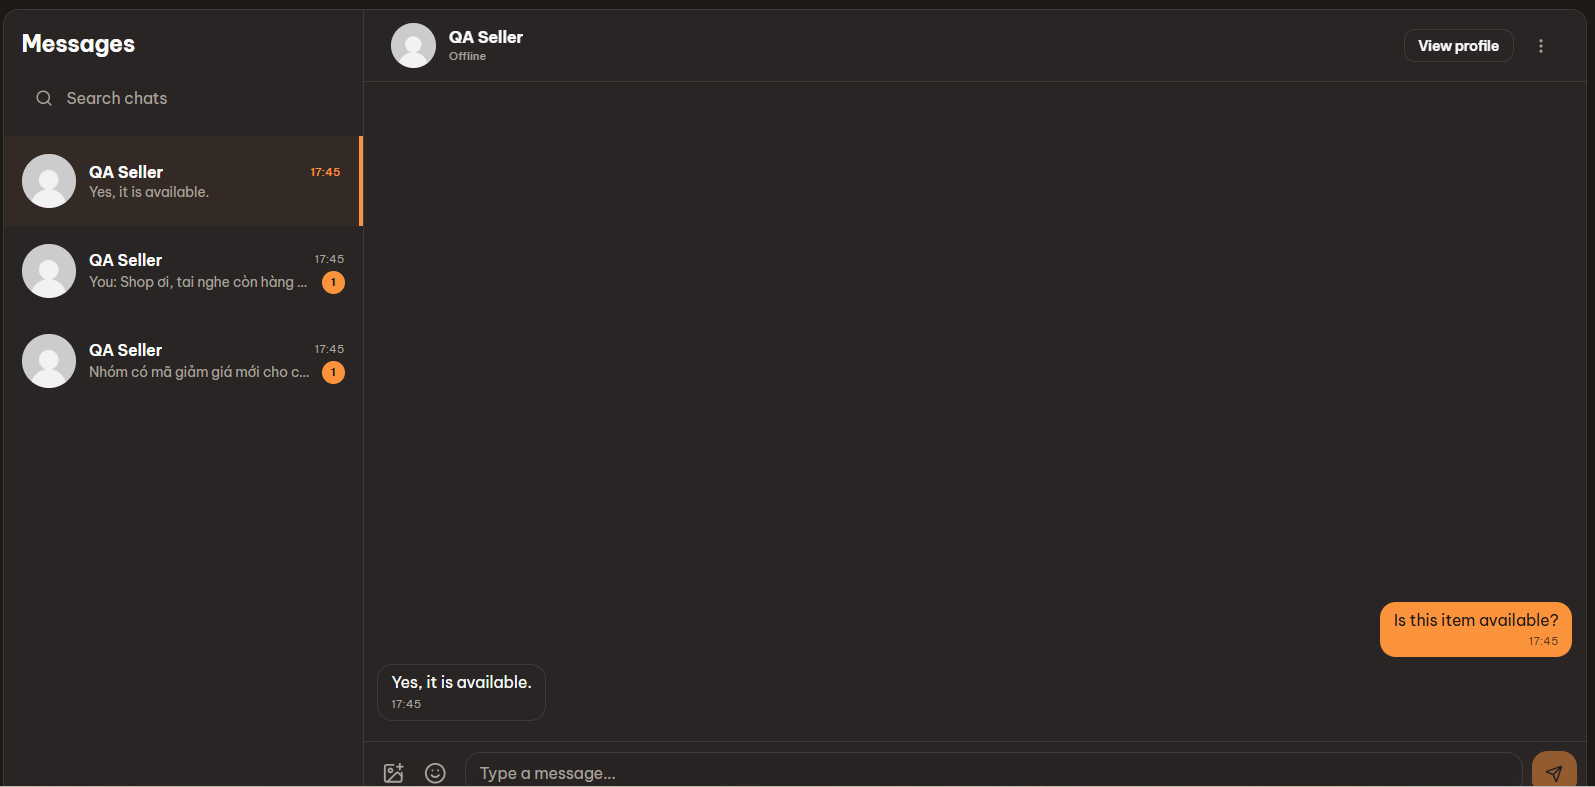
\includegraphics[width=\textwidth]{Images/UI/module2/messaging-page.png}
\caption{Giao diện trò chuyện trực tiếp}
\label{fig}
\end{figure}

\subsection{Trang Nhóm}

Chức năng nhóm cho phép người dùng tham gia vào các cộng đồng có cùng sở thích và nhu cầu trao đổi trên nền tảng Social Commerce. Hệ thống hỗ trợ tạo nhóm công khai hoặc riêng tư nhằm tăng khả năng kết nối và xây dựng cộng đồng người dùng.

Trang khám phá nhóm hiển thị danh sách các nhóm nổi bật, nhóm được đề xuất và các nhóm mà người dùng đã tham gia. Người dùng có thể tìm kiếm nhóm, xem thông tin cơ bản của từng nhóm và tham gia trực tiếp từ giao diện hệ thống.

\begin{figure}[H]
\centering
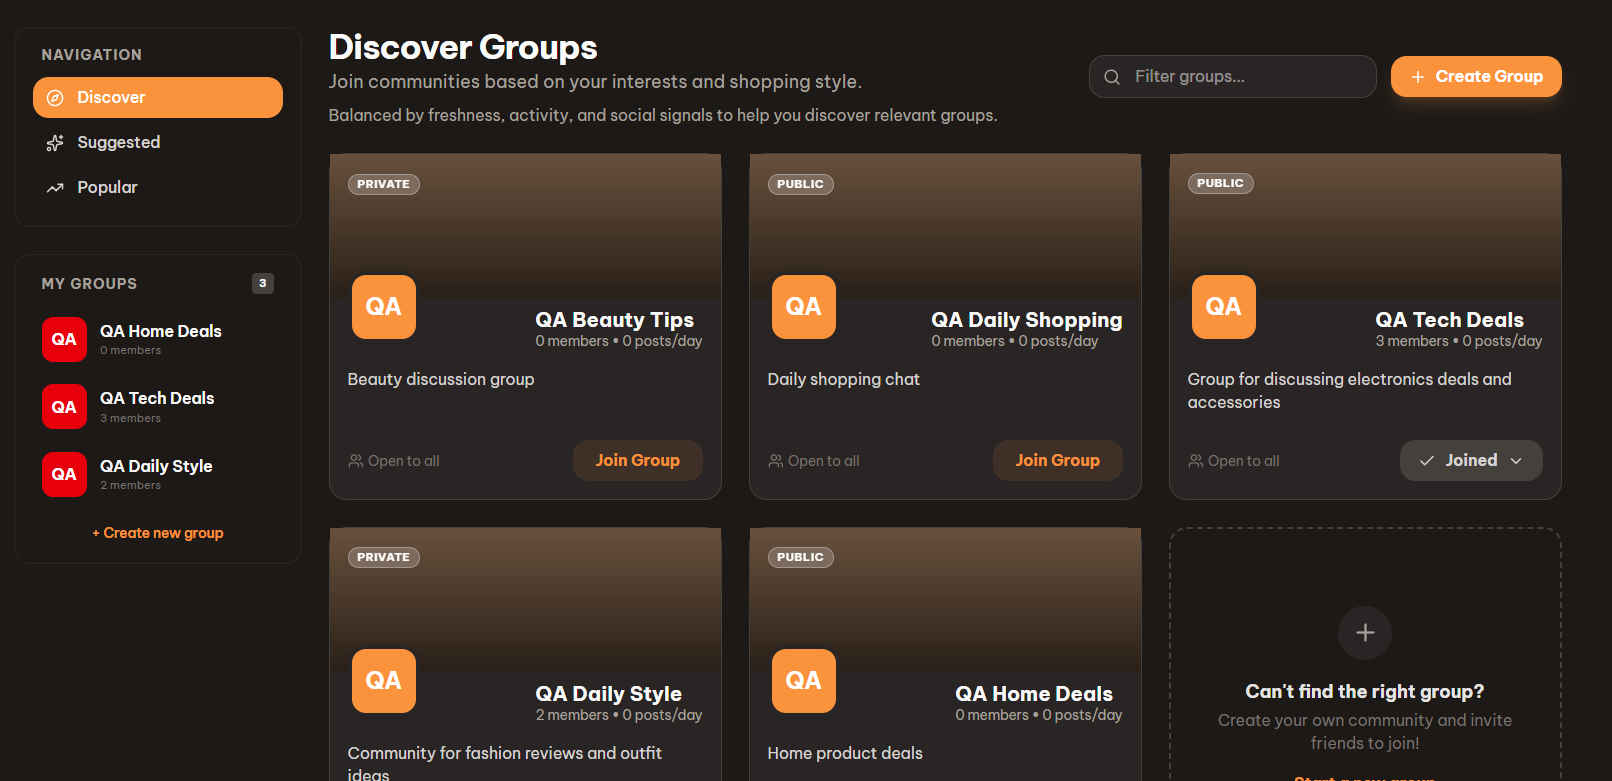
\includegraphics[width=\textwidth]{Images/UI/module2/groups-discover.png}
\caption{Giao diện khám phá nhóm}
\label{fig}
\end{figure}

Khi truy cập vào một nhóm cụ thể, hệ thống hiển thị đầy đủ các thông tin liên quan bao gồm ảnh đại diện, ảnh bìa, mô tả nhóm, danh sách thành viên và các bài đăng trong nhóm. Người dùng có thể tạo bài viết mới, chia sẻ nội dung và tương tác với các thành viên khác trong nhóm.

Ngoài ra, hệ thống còn hỗ trợ các chức năng quản lý nhóm như chỉnh sửa thông tin nhóm, thay đổi quyền riêng tư và quản lý thành viên đối với tài khoản quản trị viên nhóm.

\begin{figure}[H]
\centering
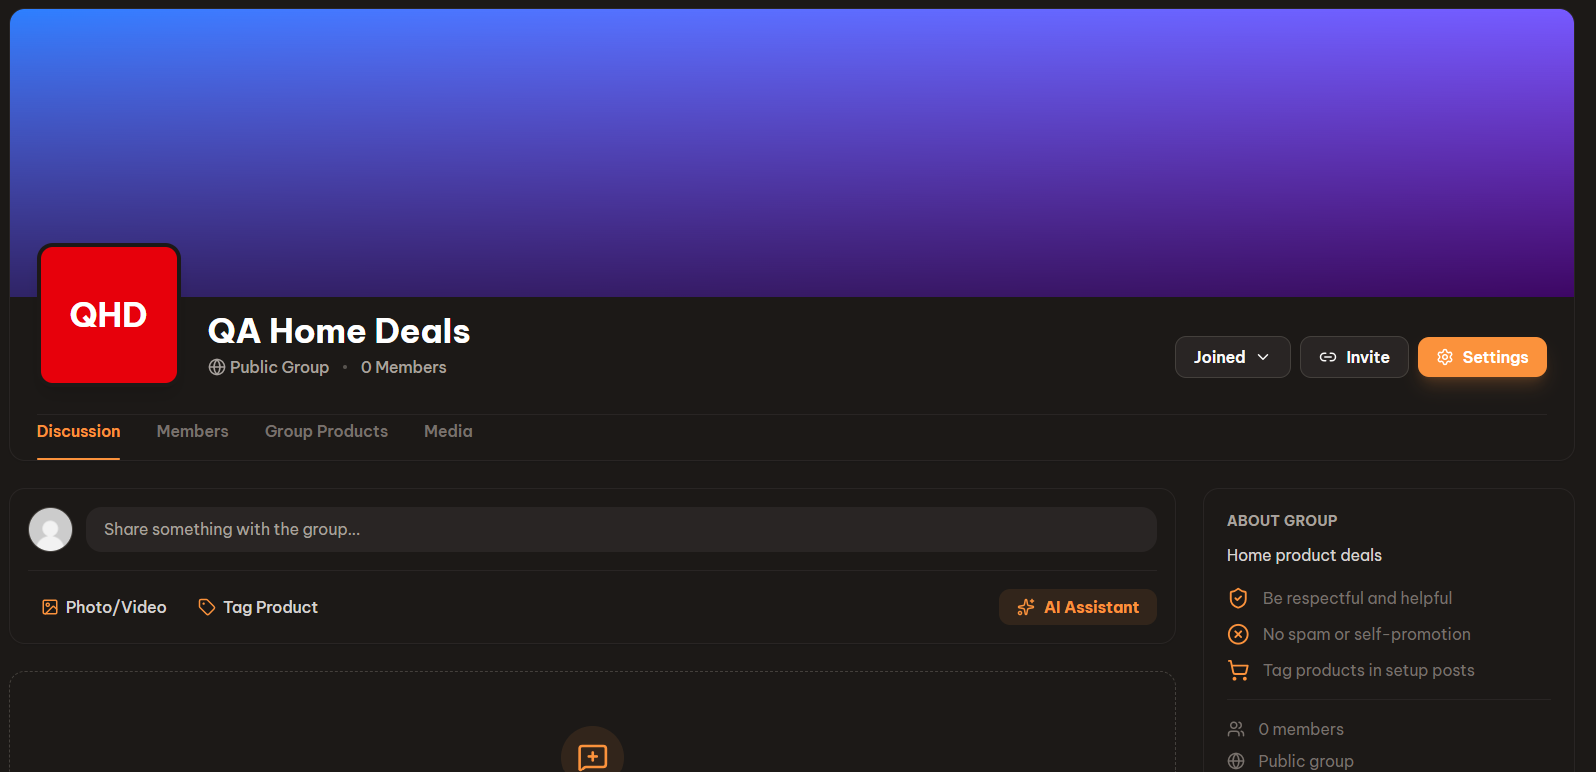
\includegraphics[width=\textwidth]{Images/UI/module2/group-detail.png}
\caption{Giao diện chi tiết nhóm}
\label{fig}
\end{figure}

\begin{figure}[H]
\centering
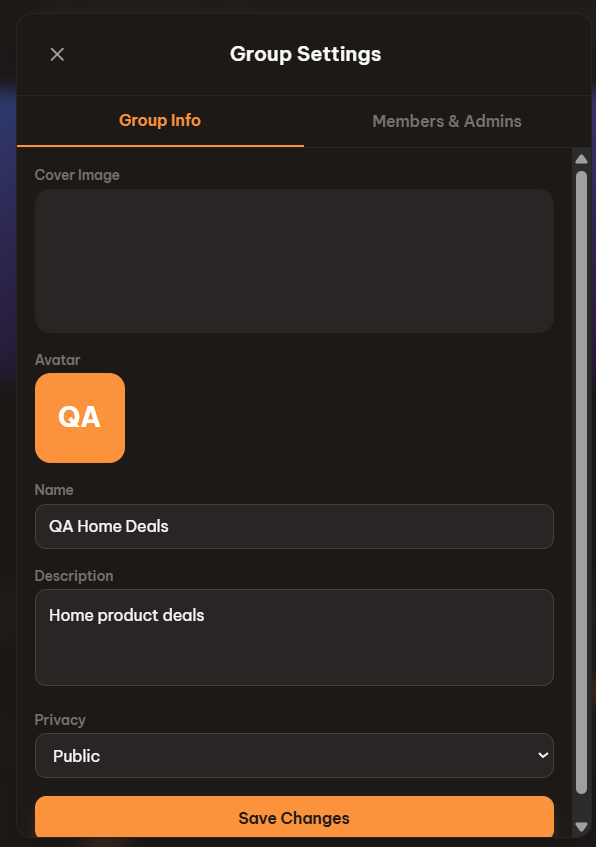
\includegraphics[width=\textwidth]{Images/UI/module2/group-settings.png}
\caption{Giao diện quản lý thông tin nhóm}
\label{fig}
\end{figure}

\subsection{Trang Tìm kiếm}

Chức năng tìm kiếm cho phép người dùng tra cứu các nội dung trên nền tảng Social Commerce bao gồm sản phẩm, bài đăng và người dùng. Hệ thống hỗ trợ tìm kiếm theo từ khóa kết hợp với cơ chế phân loại kết quả nhằm giúp người dùng dễ dàng tiếp cận nội dung phù hợp.

Giao diện tìm kiếm được tổ chức theo từng danh mục kết quả như tất cả kết quả, sản phẩm, bài đăng và người dùng. Người dùng có thể chuyển đổi nhanh giữa các danh mục để xem nội dung liên quan đến từ khóa tìm kiếm.

Đối với tìm kiếm sản phẩm, hệ thống hỗ trợ thêm các bộ lọc và sắp xếp kết quả như khoảng giá, đánh giá sản phẩm và độ liên quan của kết quả tìm kiếm. Người dùng cũng có thể sắp xếp sản phẩm theo mức độ phổ biến, mới nhất hoặc giá bán nhằm tối ưu trải nghiệm mua sắm trên nền tảng.

\begin{figure}[H]
\centering
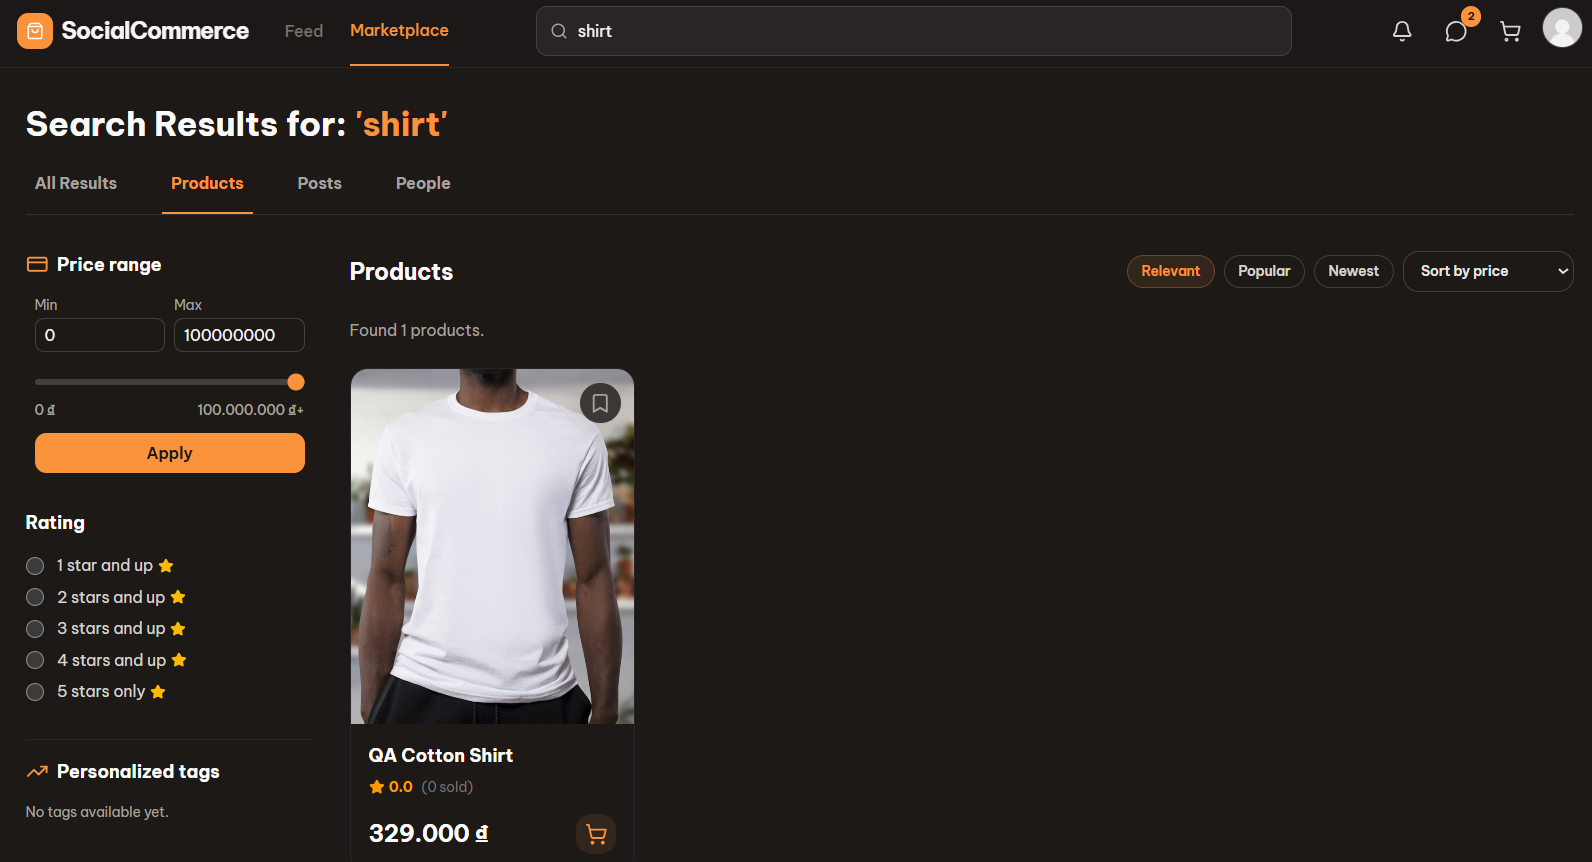
\includegraphics[width=\textwidth]{Images/UI/module2/search-page.png}
\caption{Giao diện tìm kiếm trên hệ thống}
\label{fig}
\end{figure}

\section{Module 3: Hoạt động Thương mại}

Module hoạt động thương mại là thành phần cốt lõi của hệ thống Social Commerce, hỗ trợ các chức năng liên quan đến mua bán sản phẩm, quản lý cửa hàng, xử lý đơn hàng và theo dõi hoạt động kinh doanh trên nền tảng.

Hệ thống cho phép người dùng khám phá sản phẩm, tìm kiếm và lọc sản phẩm theo nhiều tiêu chí khác nhau, thêm sản phẩm vào giỏ hàng, thực hiện thanh toán và theo dõi trạng thái đơn hàng. Đối với người bán, hệ thống cung cấp các công cụ quản lý cửa hàng, quản lý sản phẩm, theo dõi doanh thu và xử lý đơn hàng trực tiếp trên nền tảng.

\subsection{Trang Khám phá Sản phẩm}

Trang khám phá sản phẩm hiển thị danh sách các sản phẩm đang được kinh doanh trên nền tảng dưới dạng lưới trực quan. Mỗi sản phẩm bao gồm hình ảnh, tên sản phẩm, giá bán, đánh giá và các thông tin liên quan nhằm hỗ trợ người dùng dễ dàng tham khảo và lựa chọn sản phẩm phù hợp.

Hệ thống hỗ trợ tìm kiếm và lọc sản phẩm theo nhiều tiêu chí như khoảng giá, đánh giá, mức độ phổ biến và thời gian đăng tải. Ngoài ra, người dùng có thể lưu sản phẩm yêu thích, xem nhanh thông tin sản phẩm và truy cập trực tiếp đến trang chi tiết sản phẩm từ giao diện khám phá.

Dữ liệu sản phẩm được tải động kết hợp với cơ chế phân trang và sắp xếp nhằm tối ưu hiệu năng hiển thị và trải nghiệm mua sắm trên nền tảng.

\begin{figure}[H]
\centering
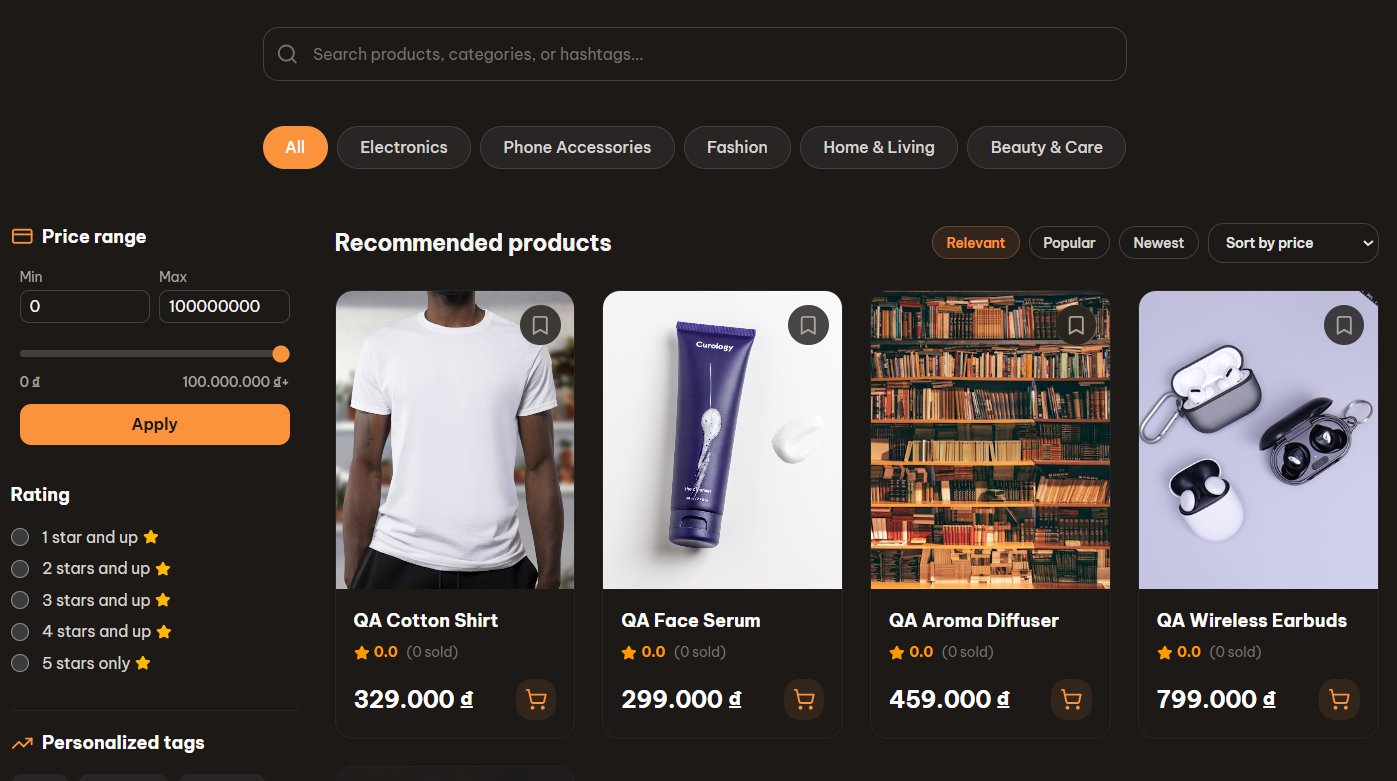
\includegraphics[width=\textwidth]{Images/UI/module3/product-explore.png}
\caption{Giao diện khám phá sản phẩm}
\label{fig:module3-product-explore}
\end{figure}

\subsection{Trang Chi tiết Sản phẩm}

Trang chi tiết sản phẩm cung cấp đầy đủ thông tin liên quan đến một sản phẩm cụ thể bao gồm hình ảnh, mô tả, giá bán, thông tin cửa hàng và đánh giá từ người mua. Người dùng có thể xem nhiều hình ảnh sản phẩm, lựa chọn biến thể sản phẩm và thực hiện các thao tác mua hàng trực tiếp từ giao diện này.

Hệ thống đồng thời hỗ trợ hiển thị đánh giá sản phẩm, số lượng đã bán, thông tin người bán và các sản phẩm liên quan nhằm tăng trải nghiệm mua sắm và hỗ trợ người dùng trong quá trình tham khảo sản phẩm.

Ngoài ra, người dùng có thể thêm sản phẩm vào giỏ hàng, lưu sản phẩm yêu thích hoặc chia sẻ sản phẩm trực tiếp thông qua giao diện chi tiết sản phẩm.

\begin{figure}[H]
\centering
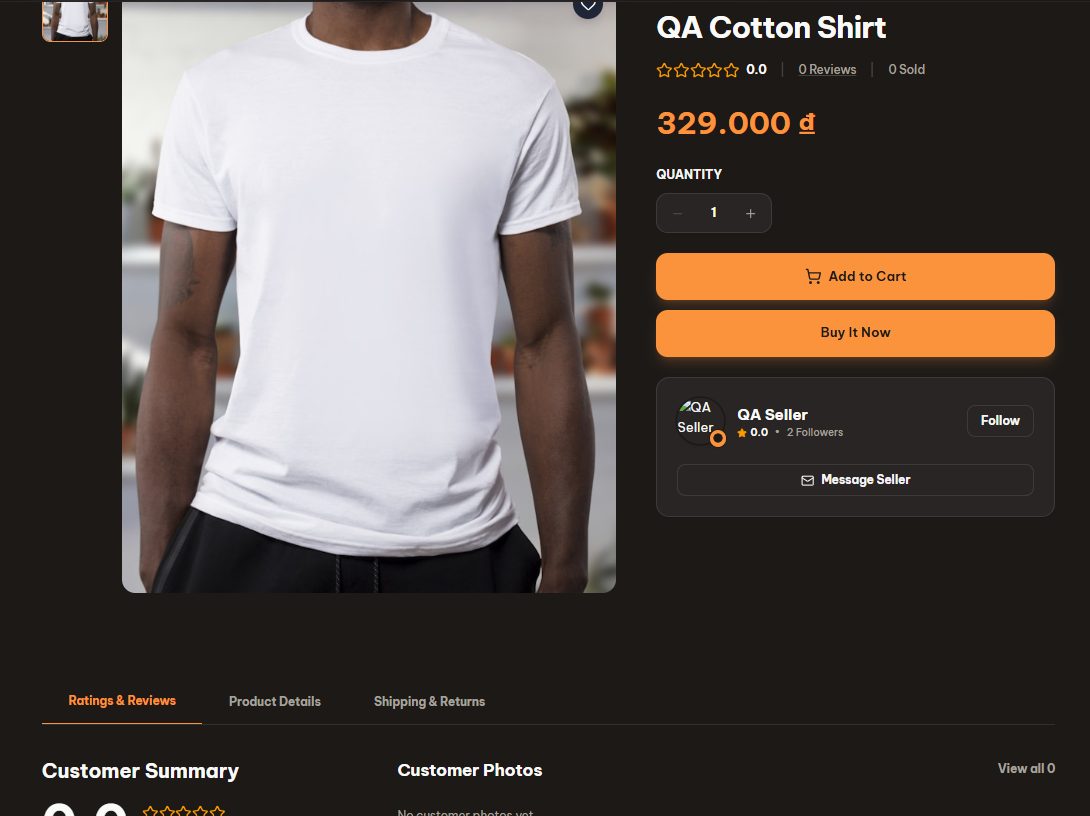
\includegraphics[width=\textwidth]{Images/UI/module3/product-detail.png}
\caption{Giao diện chi tiết sản phẩm}
\label{fig:module3-product-detail}
\end{figure}

\subsubsection{Trang Giỏ hàng}

Trang giỏ hàng cho phép người dùng quản lý các sản phẩm đã lựa chọn trước khi thực hiện thanh toán. Hệ thống hiển thị đầy đủ thông tin của từng sản phẩm bao gồm hình ảnh, tên sản phẩm, giá bán, số lượng và tổng giá trị đơn hàng.

Người dùng có thể thay đổi số lượng sản phẩm, xóa sản phẩm khỏi giỏ hàng hoặc tiếp tục mua sắm trực tiếp từ giao diện này. Hệ thống đồng thời tự động cập nhật tổng tiền dựa trên các thay đổi trong giỏ hàng nhằm hỗ trợ người dùng dễ dàng theo dõi chi phí đơn hàng.

Ngoài ra, giỏ hàng còn hỗ trợ lưu trạng thái sản phẩm theo tài khoản người dùng nhằm đảm bảo dữ liệu được đồng bộ giữa các phiên đăng nhập khác nhau trên hệ thống.

\begin{figure}[H]
\centering
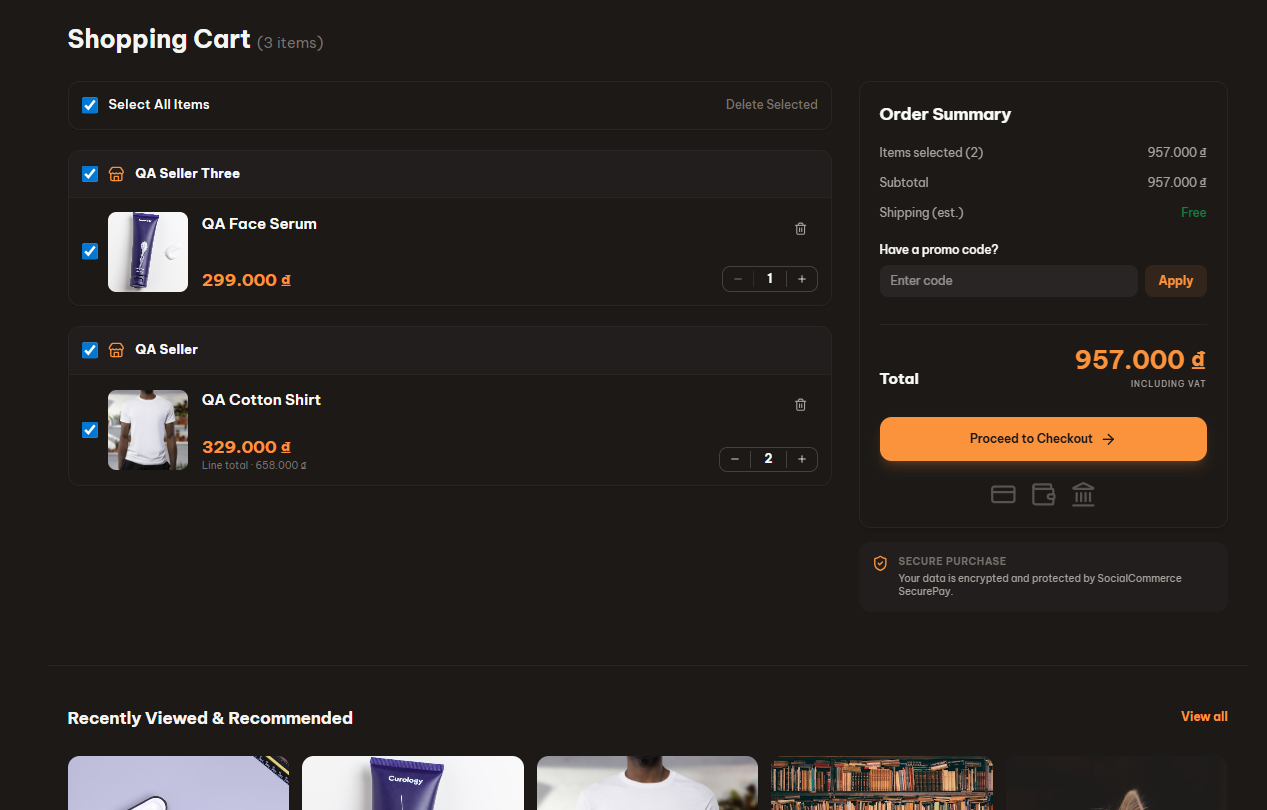
\includegraphics[width=\textwidth]{Images/UI/module3/cart-page.png}
\caption{Giao diện giỏ hàng}
\label{fig:module3-cart-page}
\end{figure}

\subsubsection{Trang Thanh toán}

Trang thanh toán hỗ trợ người dùng hoàn tất quá trình đặt hàng thông qua quy trình xác nhận đơn hàng trực quan và thuận tiện. Hệ thống hiển thị thông tin sản phẩm, địa chỉ giao hàng, phương thức thanh toán và tổng giá trị đơn hàng trước khi xác nhận thanh toán.

Người dùng có thể lựa chọn hoặc cập nhật địa chỉ nhận hàng, kiểm tra thông tin sản phẩm và xác nhận đơn hàng trực tiếp trên giao diện thanh toán. Sau khi thanh toán thành công, hệ thống sẽ tạo đơn hàng và cập nhật trạng thái đơn hàng tương ứng trong cơ sở dữ liệu.

Quy trình thanh toán được xây dựng theo từng bước nhằm giúp người dùng dễ dàng theo dõi thông tin và hạn chế sai sót trong quá trình đặt hàng.

\begin{figure}[H]
\centering
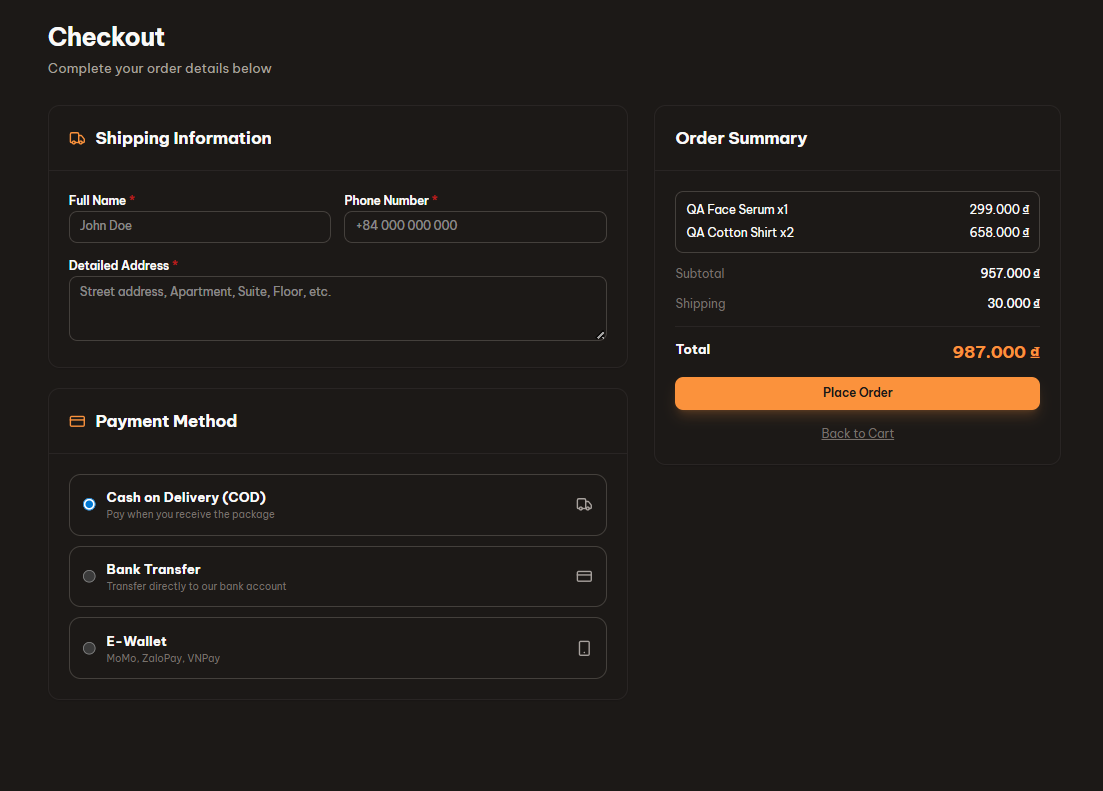
\includegraphics[width=\textwidth]{Images/UI/module3/checkout-page.png}
\caption{Giao diện thanh toán đơn hàng}
\label{fig:module3-checkout-page}
\end{figure}

\subsubsection{Trang Quản lý Cửa hàng}

Trang quản lý cửa hàng cung cấp giao diện tổng quan dành cho người bán nhằm theo dõi hoạt động kinh doanh trên nền tảng. Hệ thống hỗ trợ quản lý sản phẩm, quản lý đơn hàng và theo dõi các thống kê liên quan đến hoạt động bán hàng.

Người bán có thể xem nhanh số lượng đơn hàng, doanh thu, trạng thái sản phẩm và các thông tin thống kê trực tiếp từ giao diện quản lý. Ngoài ra, hệ thống còn hỗ trợ điều hướng nhanh đến các chức năng quản lý sản phẩm và xử lý đơn hàng nhằm tối ưu quá trình vận hành cửa hàng.

Giao diện dashboard được xây dựng theo hướng trực quan, hỗ trợ hiển thị dữ liệu thống kê và hoạt động kinh doanh theo thời gian thực.

\begin{figure}[H]
\centering
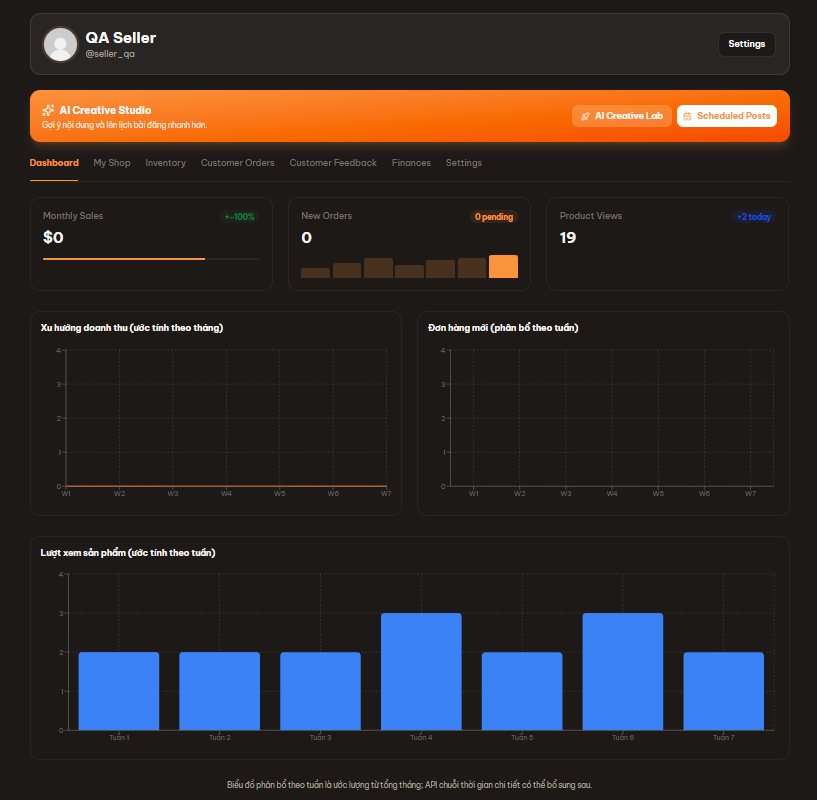
\includegraphics[width=\textwidth]{Images/UI/module3/seller-dashboard.png}
\caption{Giao diện quản lý cửa hàng}
\label{fig:module3-seller-dashboard}
\end{figure}

\subsubsection{Trang Cửa hàng của tôi}

Trang “Cửa hàng của tôi” cho phép người bán quản lý toàn bộ danh sách sản phẩm đang kinh doanh trên nền tảng Social Commerce. Giao diện hiển thị thông tin tổng quan của cửa hàng cùng danh sách sản phẩm, trạng thái hoạt động và các chỉ số liên quan đến quá trình kinh doanh.

Người bán có thể tìm kiếm sản phẩm theo tên, lọc sản phẩm theo trạng thái như đang hoạt động, bản nháp, hết hàng hoặc đã lưu trữ. Ngoài ra, hệ thống còn hỗ trợ sắp xếp danh sách sản phẩm và hiển thị các thông tin thống kê như lượt xem, số lượng đã bán và trạng thái hiện tại của từng sản phẩm.

Từ giao diện này, người bán có thể nhanh chóng thực hiện các thao tác quản lý như thêm sản phẩm mới, chỉnh sửa thông tin sản phẩm, lưu trữ sản phẩm hoặc xóa sản phẩm khỏi hệ thống.

\begin{figure}[H]
\centering
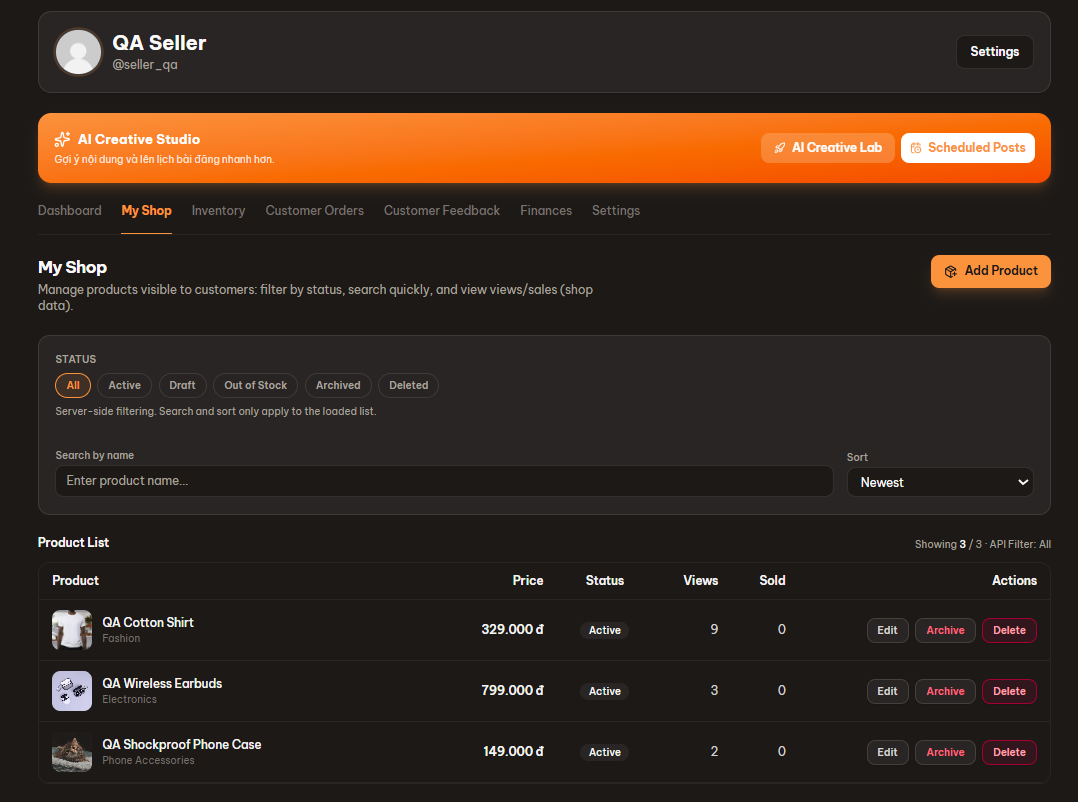
\includegraphics[width=\textwidth]{Images/UI/module3/my-shop.png}
\caption{Giao diện quản lý sản phẩm trong cửa hàng}
\label{fig}
\end{figure}

\subsubsection{Trang Tạo và Chỉnh sửa Sản phẩm}

Chức năng tạo và chỉnh sửa sản phẩm cho phép người bán quản lý thông tin sản phẩm trực tiếp trên nền tảng Social Commerce. Người bán có thể tạo mới sản phẩm hoặc cập nhật các thông tin liên quan như tên sản phẩm, mô tả, giá bán, danh mục, hình ảnh và trạng thái hiển thị của sản phẩm.

Hệ thống hỗ trợ tải lên nhiều hình ảnh sản phẩm nhằm tăng khả năng hiển thị và hỗ trợ người mua dễ dàng tham khảo thông tin trước khi đưa ra quyết định mua hàng. Các hình ảnh sản phẩm được lưu trữ thông qua Cloudinary để tối ưu khả năng quản lý và hiển thị dữ liệu đa phương tiện.

Ngoài ra, hệ thống còn hỗ trợ cập nhật nhanh thông tin sản phẩm và đồng bộ dữ liệu trực tiếp trên giao diện quản lý cửa hàng của người bán.

\begin{figure}[H]
\centering
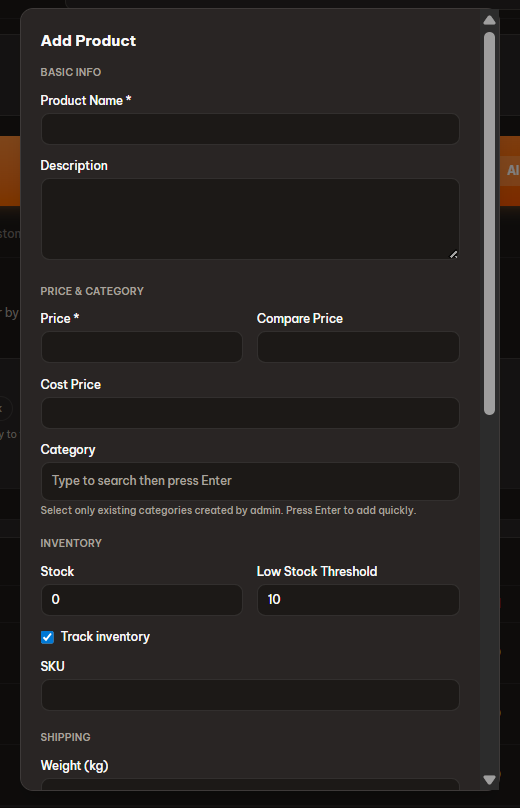
\includegraphics[width=\textwidth]{Images/UI/module3/create-product.png}
\caption{Giao diện tạo và chỉnh sửa sản phẩm}
\label{fig:module3-create-product}
\end{figure}

\subsubsection{Trang Quản lý Đơn hàng}

Trang quản lý đơn hàng cho phép người bán theo dõi và xử lý các đơn hàng phát sinh trên hệ thống. Giao diện hiển thị danh sách đơn hàng cùng với các thông tin quan trọng như mã đơn hàng, người mua, trạng thái đơn hàng, thời gian đặt hàng và tổng giá trị thanh toán.

Hệ thống hỗ trợ quản lý nhiều trạng thái đơn hàng khác nhau bao gồm chờ xác nhận, đang xử lý, đang giao hàng, đã hoàn thành và đã hủy. Người bán có thể cập nhật trạng thái đơn hàng trực tiếp từ giao diện quản lý nhằm đồng bộ tiến trình xử lý với người mua.

Ngoài ra, hệ thống còn hỗ trợ tìm kiếm và lọc đơn hàng nhằm giúp người bán dễ dàng quản lý số lượng lớn đơn hàng trên nền tảng.

\begin{figure}[H]
\centering
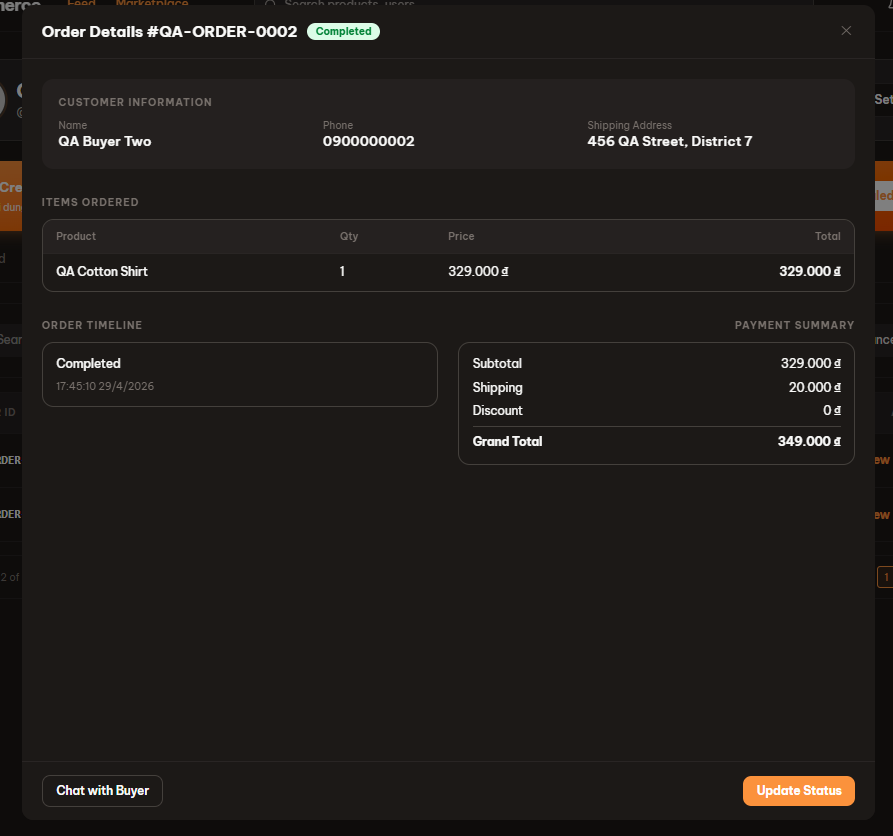
\includegraphics[width=\textwidth]{Images/UI/module3/orders-management.png}
\caption{Giao diện quản lý đơn hàng}
\label{fig:module3-orders-management}
\end{figure}


\section{Module 4: Hệ thống Quản trị}

Module quản trị được xây dựng như một hệ thống riêng biệt nhằm hỗ trợ quản trị viên theo dõi và quản lý toàn bộ hoạt động của nền tảng Social Commerce. Hệ thống quản trị sử dụng backend và frontend độc lập với hệ thống người dùng thông thường, đồng thời kết nối chung cơ sở dữ liệu để thực hiện các chức năng kiểm duyệt và vận hành hệ thống.

\subsubsection{Trang Đăng nhập Quản trị}

Trang đăng nhập quản trị cho phép quản trị viên truy cập vào hệ thống admin thông qua tài khoản quản trị riêng. Sau khi xác thực thành công, quản trị viên có thể sử dụng các chức năng quản lý người dùng, nội dung, danh mục sản phẩm và xử lý báo cáo trên hệ thống.

\begin{figure}[H]
\centering
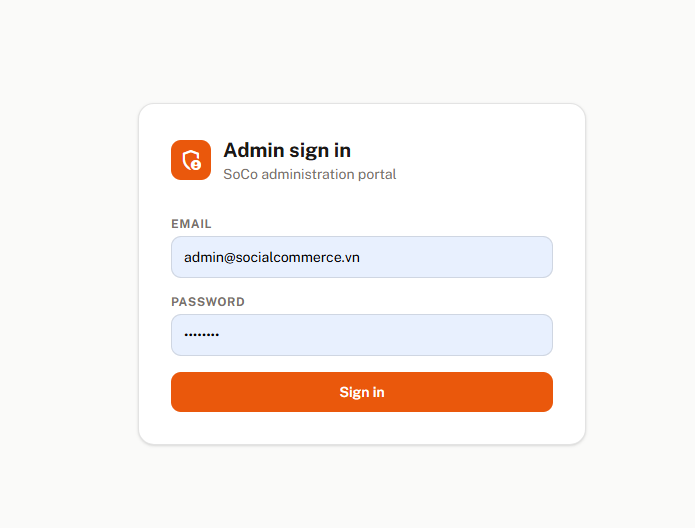
\includegraphics[width=\textwidth]{Images/UI/module4/admin-login.png}
\caption{Giao diện đăng nhập quản trị}
\label{fig:module4-admin-login}
\end{figure}

\subsubsection{Trang Dashboard Quản trị}

Trang dashboard quản trị hiển thị tổng quan các thông tin và thống kê quan trọng của hệ thống bao gồm số lượng người dùng, sản phẩm, đơn hàng và các hoạt động phát sinh trên nền tảng.

Hệ thống hỗ trợ hiển thị dữ liệu thống kê trực quan nhằm giúp quản trị viên dễ dàng theo dõi tình trạng hoạt động của hệ thống và phát hiện các vấn đề cần xử lý. Ngoài ra, dashboard còn hỗ trợ điều hướng nhanh đến các chức năng quản lý chính của hệ thống quản trị.

\begin{figure}[H]
\centering
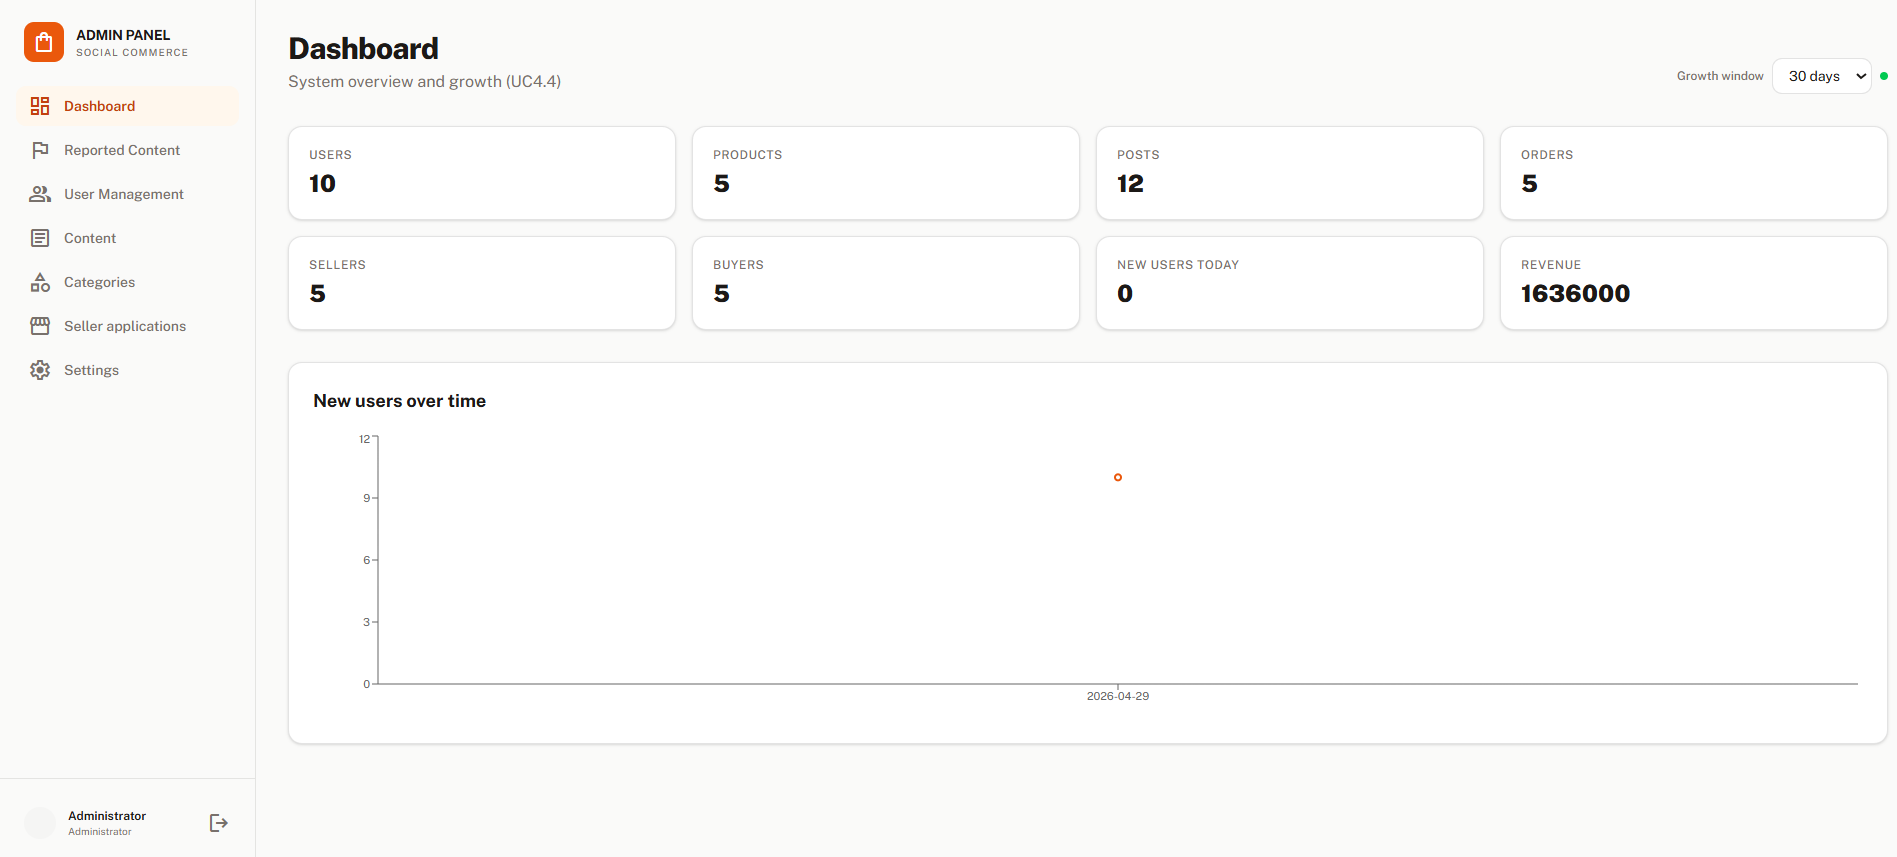
\includegraphics[width=\textwidth]{Images/UI/module4/admin-dashboard.png}
\caption{Giao diện dashboard quản trị}
\label{fig:module4-admin-dashboard}
\end{figure}

\subsubsection{Trang Quản lý Người dùng}

Trang quản lý người dùng cho phép quản trị viên theo dõi danh sách tài khoản đang hoạt động trên hệ thống. Giao diện hỗ trợ tìm kiếm, lọc và quản lý thông tin người dùng nhằm hỗ trợ quá trình vận hành nền tảng.

Quản trị viên có thể thực hiện các thao tác như xem thông tin tài khoản, khóa hoặc mở khóa tài khoản và theo dõi trạng thái hoạt động của người dùng trên hệ thống. Ngoài ra, hệ thống cũng hỗ trợ quản lý các tài khoản người bán và quá trình xét duyệt đăng ký người bán.

\begin{figure}[H]
\centering
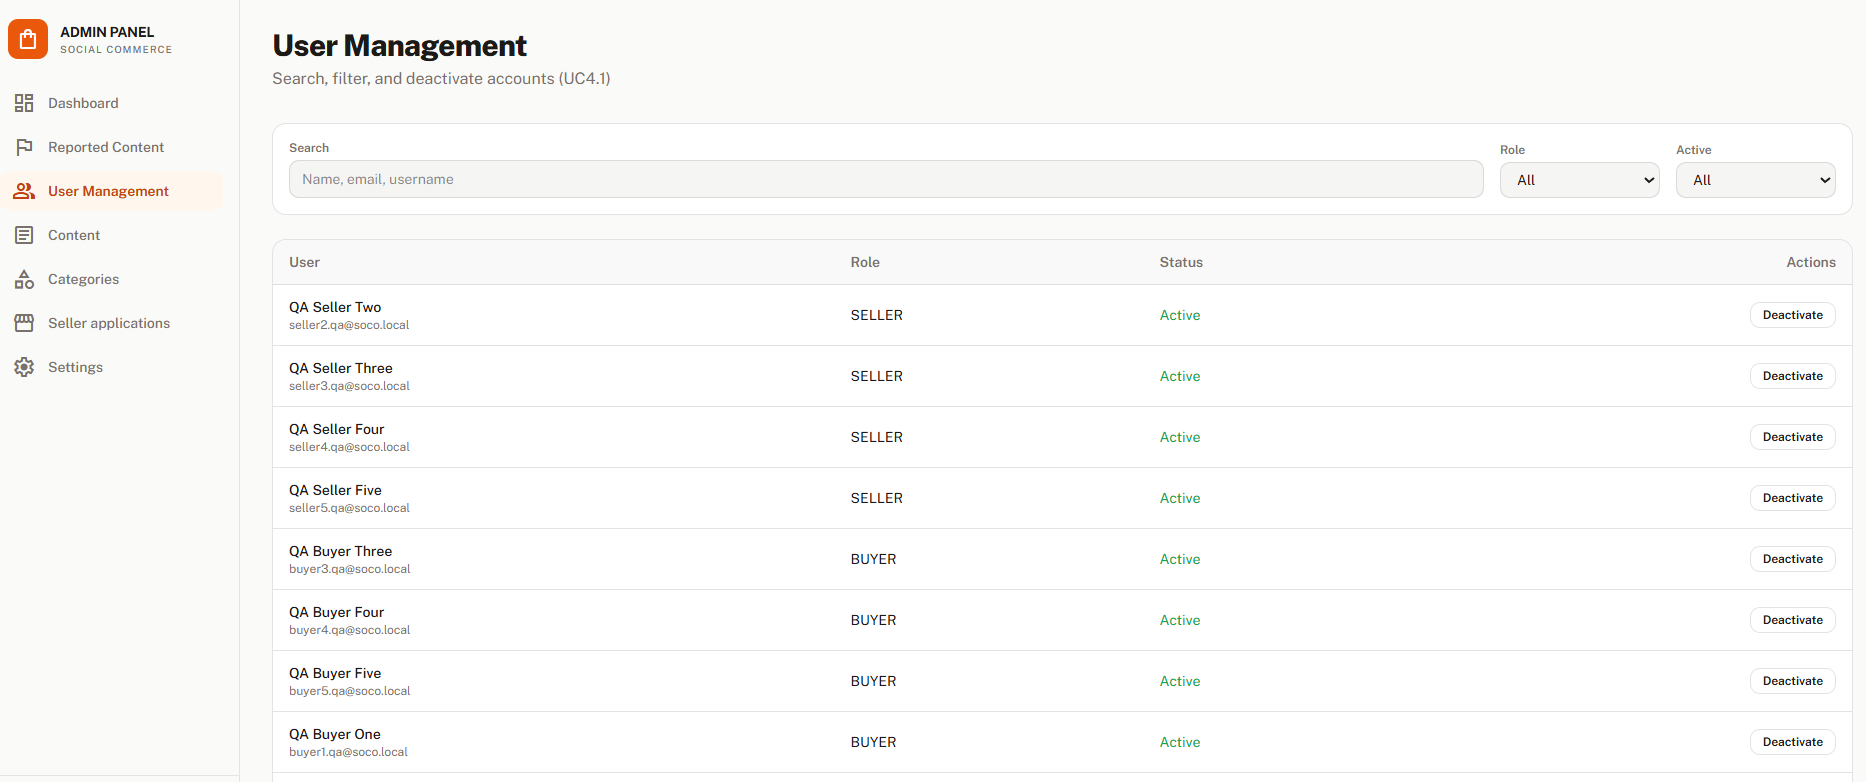
\includegraphics[width=\textwidth]{Images/UI/module4/user-management.png}
\caption{Giao diện quản lý người dùng}
\label{fig:module4-user-management}
\end{figure}

\subsubsection{Trang Quản lý Nội dung}

Trang quản lý nội dung cho phép quản trị viên theo dõi và kiểm duyệt các bài đăng và sản phẩm được đăng tải trên nền tảng. Hệ thống hỗ trợ xem nhanh nội dung, thông tin người đăng và thời gian đăng tải nhằm phục vụ cho quá trình kiểm duyệt nội dung.

Quản trị viên có thể thực hiện các hành động như xóa nội dung vi phạm hoặc xử lý các bài đăng không phù hợp với chính sách của hệ thống.

\begin{figure}[H]
\centering
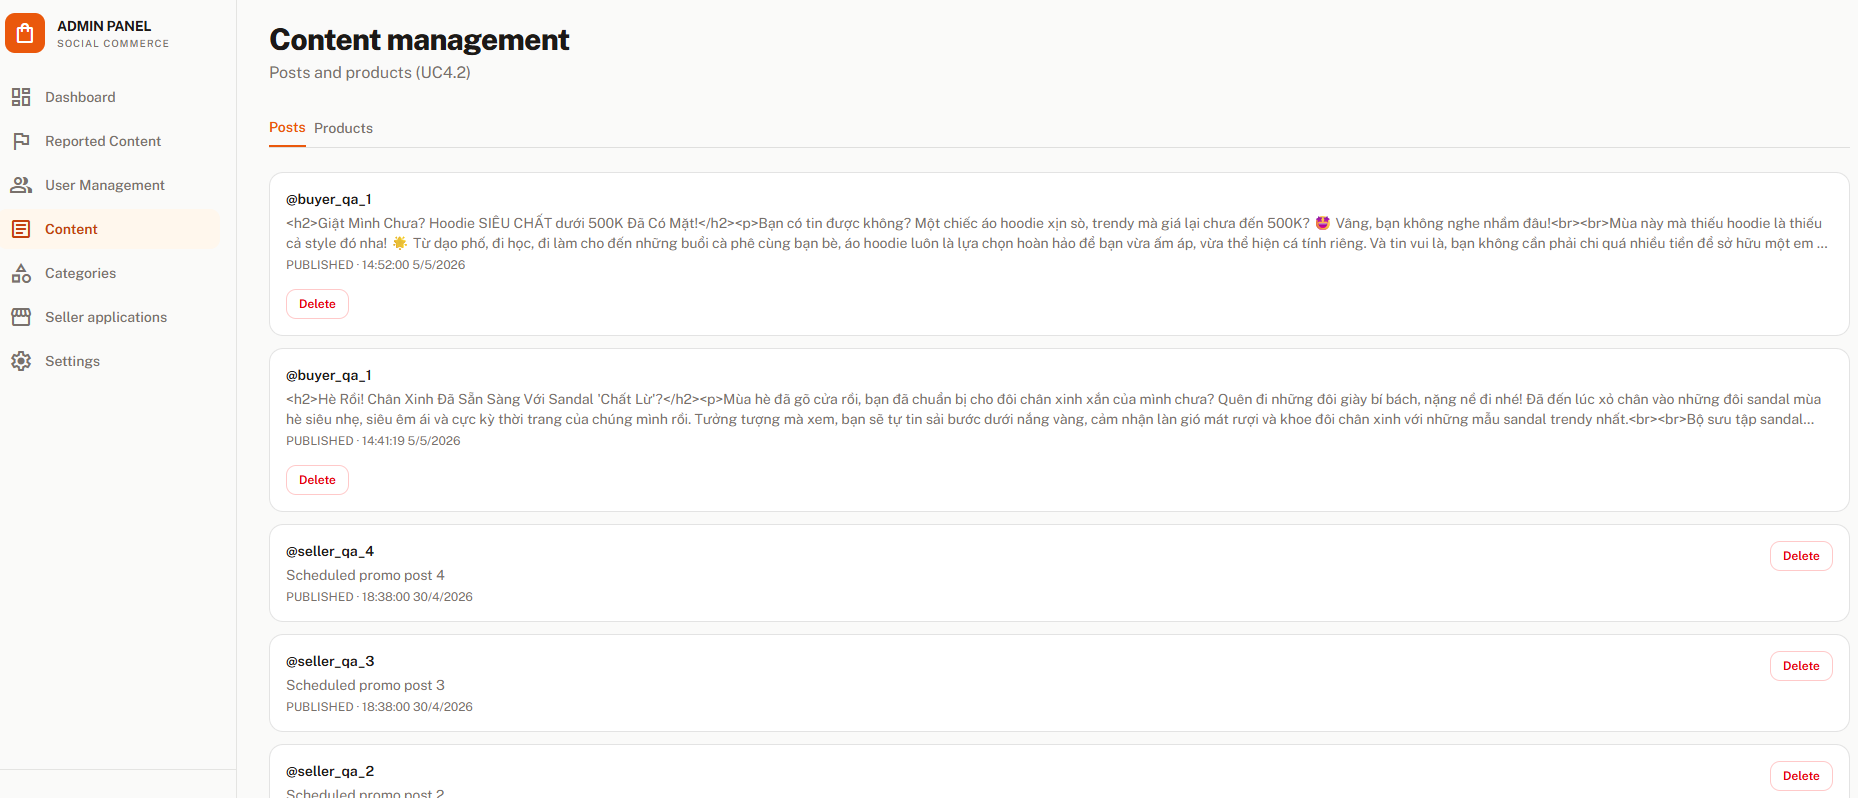
\includegraphics[width=\textwidth]{Images/UI/module4/content-management.png}
\caption{Giao diện quản lý nội dung}
\label{fig:module4-content-management}
\end{figure}

\subsubsection{Trang Quản lý Danh mục}

Trang quản lý danh mục hỗ trợ quản trị viên quản lý các danh mục sản phẩm trong marketplace. Hệ thống cho phép tạo mới, chỉnh sửa, kích hoạt hoặc vô hiệu hóa danh mục sản phẩm trực tiếp từ giao diện quản trị.

Ngoài ra, hệ thống còn hỗ trợ quản lý cấu trúc danh mục cha – con nhằm giúp tổ chức dữ liệu sản phẩm một cách trực quan và dễ quản lý hơn.

\begin{figure}[H]
\centering
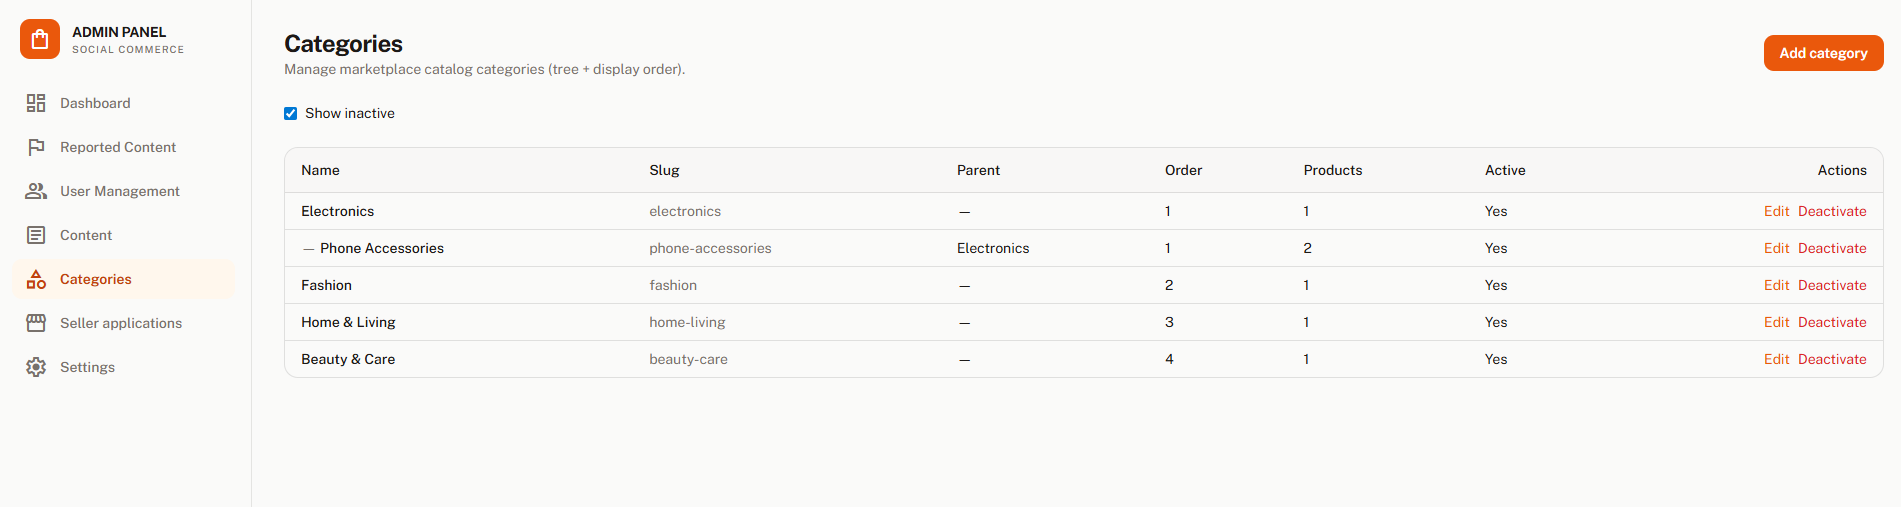
\includegraphics[width=\textwidth]{Images/UI/module4/category-management.png}
\caption{Giao diện quản lý danh mục sản phẩm}
\label{fig:module4-category-management}
\end{figure}

\subsubsection{Trang Xử lý Báo cáo}

Trang xử lý báo cáo hỗ trợ quản trị viên tiếp nhận và xử lý các báo cáo vi phạm phát sinh trên nền tảng. Hệ thống hiển thị danh sách các báo cáo liên quan đến bài đăng, sản phẩm hoặc tài khoản người dùng nhằm hỗ trợ kiểm duyệt nội dung và đảm bảo môi trường hoạt động an toàn.

Quản trị viên có thể xem chi tiết nội dung báo cáo, theo dõi trạng thái xử lý và thực hiện các hành động phù hợp như cảnh báo, ẩn nội dung hoặc khóa tài khoản vi phạm tùy theo mức độ của vấn đề được báo cáo.

\begin{figure}[H]
\centering
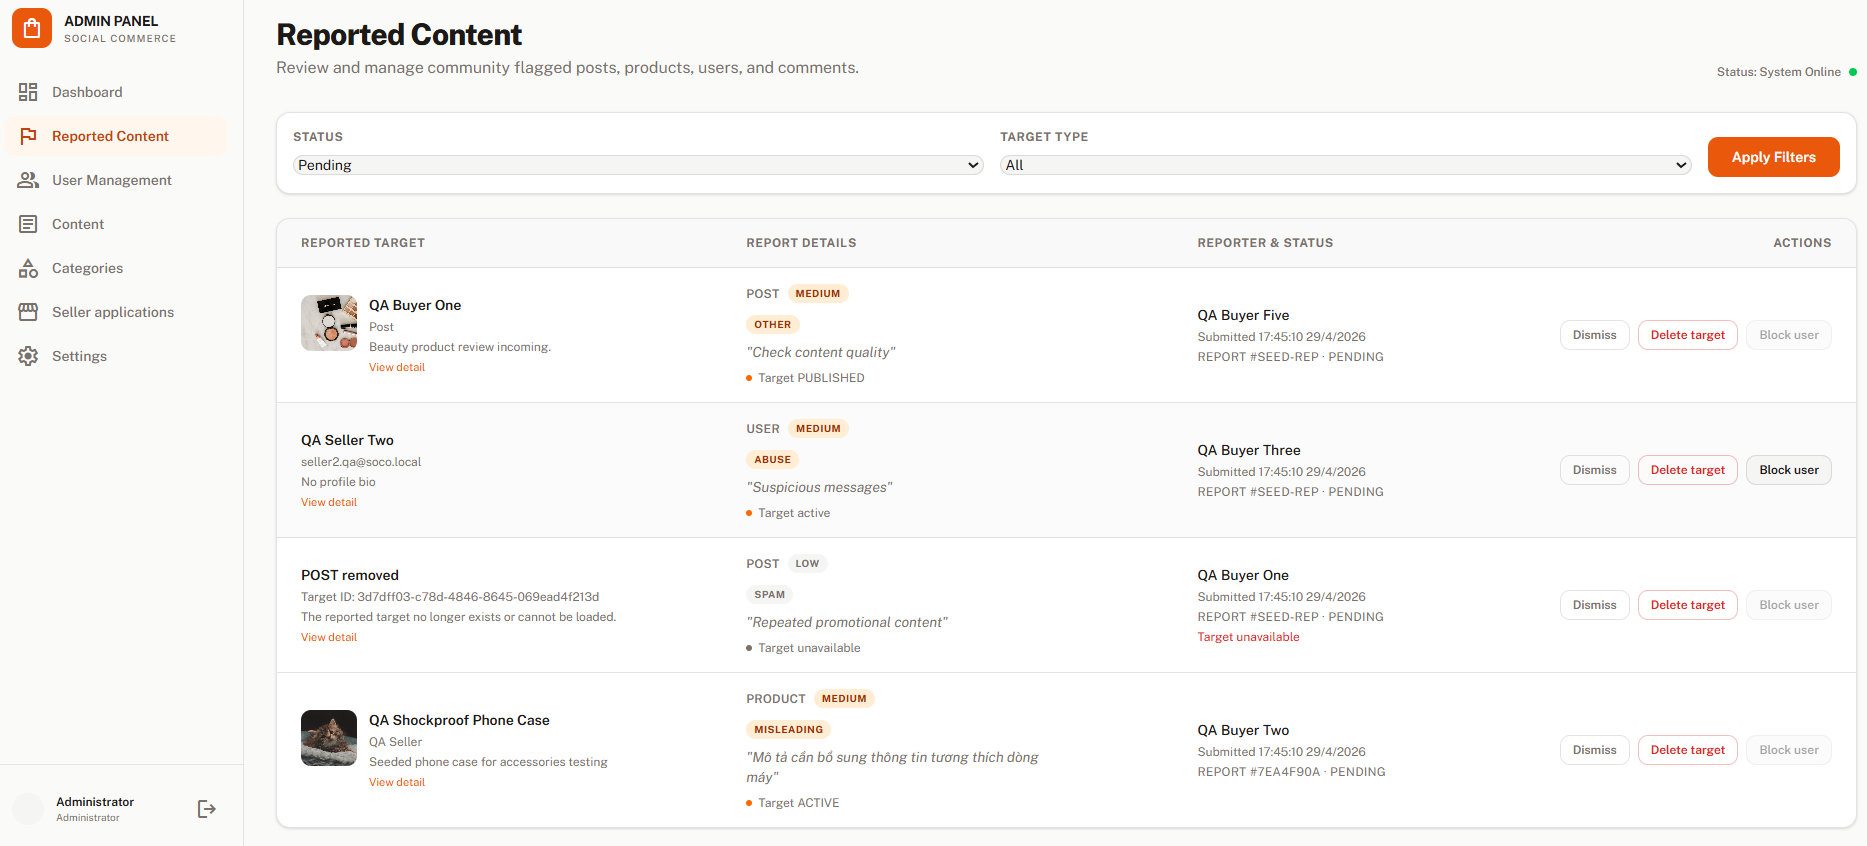
\includegraphics[width=\textwidth]{Images/UI/module4/report-management.png}
\caption{Giao diện xử lý báo cáo vi phạm}
\label{fig:module4-report-management}
\end{figure}



\section{Module 6: Quản lý Bài đăng Đã lên lịch}

Module quản lý bài đăng đã lên lịch hỗ trợ người dùng theo dõi và quản lý các bài viết được thiết lập đăng tải trong tương lai. Chức năng này được tích hợp trực tiếp với giao diện tạo bài đăng và AI Creative Studio nhằm hỗ trợ quá trình xây dựng nội dung và quản lý lịch đăng bài trên nền tảng.

\subsubsection{Trang Quản lý Bài đăng Đã lên lịch}

Trang quản lý bài đăng đã lên lịch hiển thị danh sách các bài viết đang chờ đăng tải và các bài viết đã được xuất bản trên hệ thống. Người dùng có thể xem nhanh nội dung bài viết, trạng thái bài đăng, thời gian đăng dự kiến và các thống kê liên quan trực tiếp từ giao diện quản lý.

Hệ thống hỗ trợ chỉnh sửa nội dung bài viết, thay đổi thời gian đăng hoặc hủy lịch đăng đối với các bài viết chưa được xuất bản. Ngoài ra, giao diện còn hiển thị các thống kê nhanh như số lượng bài viết sắp đăng, bài viết đã đăng và hoạt động đăng bài trong tuần nhằm hỗ trợ người dùng quản lý nội dung hiệu quả hơn.

\begin{figure}[H]
\centering
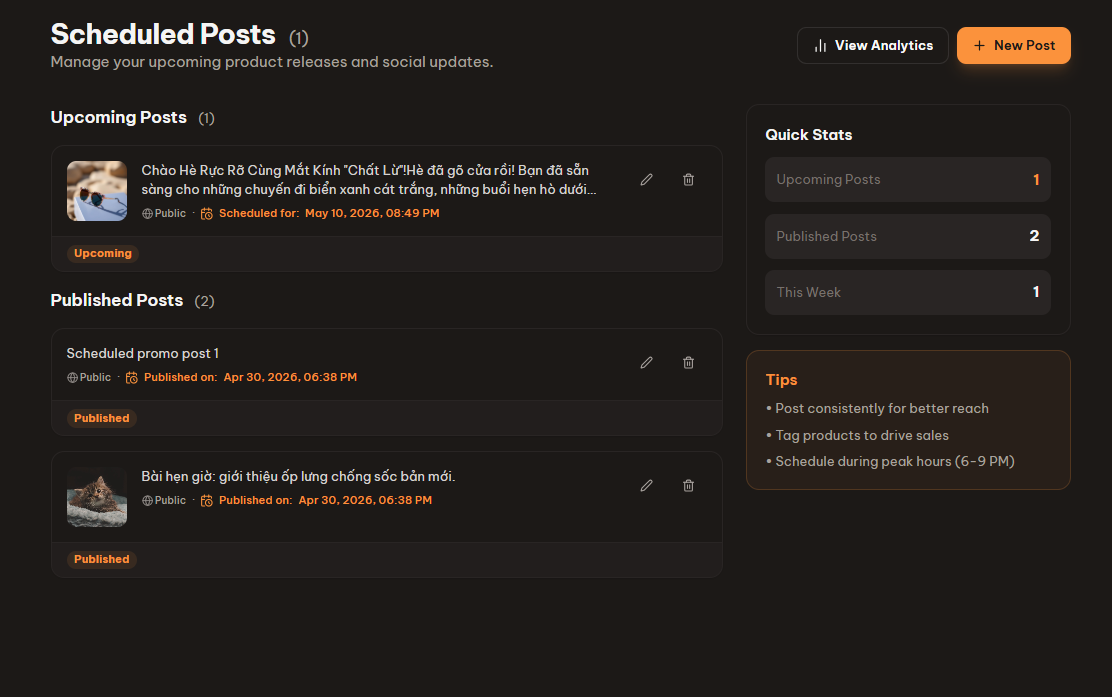
\includegraphics[width=\textwidth]{Images/UI/module6/scheduled-posts.png}
\caption{Giao diện quản lý bài đăng đã lên lịch}
\label{fig:module6-scheduled-posts}
\end{figure}

Người dùng cũng có thể chỉnh sửa bài đăng đã lên lịch trực tiếp thông qua giao diện chỉnh sửa bài viết. Hệ thống hỗ trợ thay đổi nội dung bài đăng, cấu hình AI Creative Lab và cập nhật thời gian đăng bài thông qua giao diện lịch trực quan.

\begin{figure}[H]
\centering
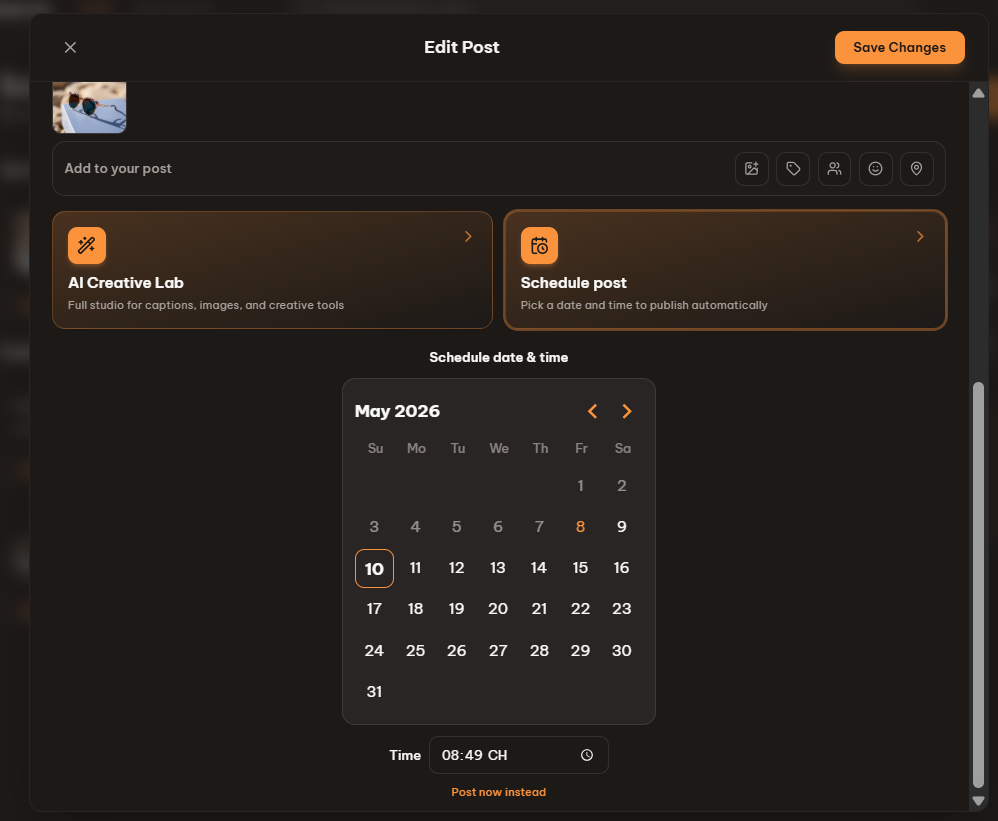
\includegraphics[width=\textwidth]{Images/UI/module6/edit-scheduled-post.png}
\caption{Giao diện chỉnh sửa bài đăng đã lên lịch}
\label{fig:module6-edit-scheduled-post}
\end{figure}


\section{Module 7: Hệ thống Thông báo}

Module thông báo hỗ trợ người dùng theo dõi các hoạt động và sự kiện mới phát sinh trên nền tảng Social Commerce. Hệ thống thông báo được xây dựng nhằm tăng khả năng tương tác giữa người dùng, đồng thời hỗ trợ cập nhật nhanh các hoạt động liên quan đến bài đăng, tin nhắn, đơn hàng và các sự kiện hệ thống.

\subsubsection{Trang Thông báo}

Trang thông báo hiển thị danh sách các thông báo phát sinh trong quá trình sử dụng hệ thống. Các thông báo được phân loại theo từng nhóm chức năng như tương tác bài viết, hoạt động thương mại, tin nhắn và thông báo hệ thống nhằm giúp người dùng dễ dàng theo dõi nội dung quan trọng.

Người dùng có thể xem trạng thái thông báo, đánh dấu đã đọc hoặc truy cập trực tiếp đến nội dung liên quan từ giao diện thông báo. Hệ thống đồng thời hỗ trợ cập nhật dữ liệu động nhằm đảm bảo các thông báo mới được hiển thị nhanh chóng trên nền tảng.

\begin{figure}[H]
\centering
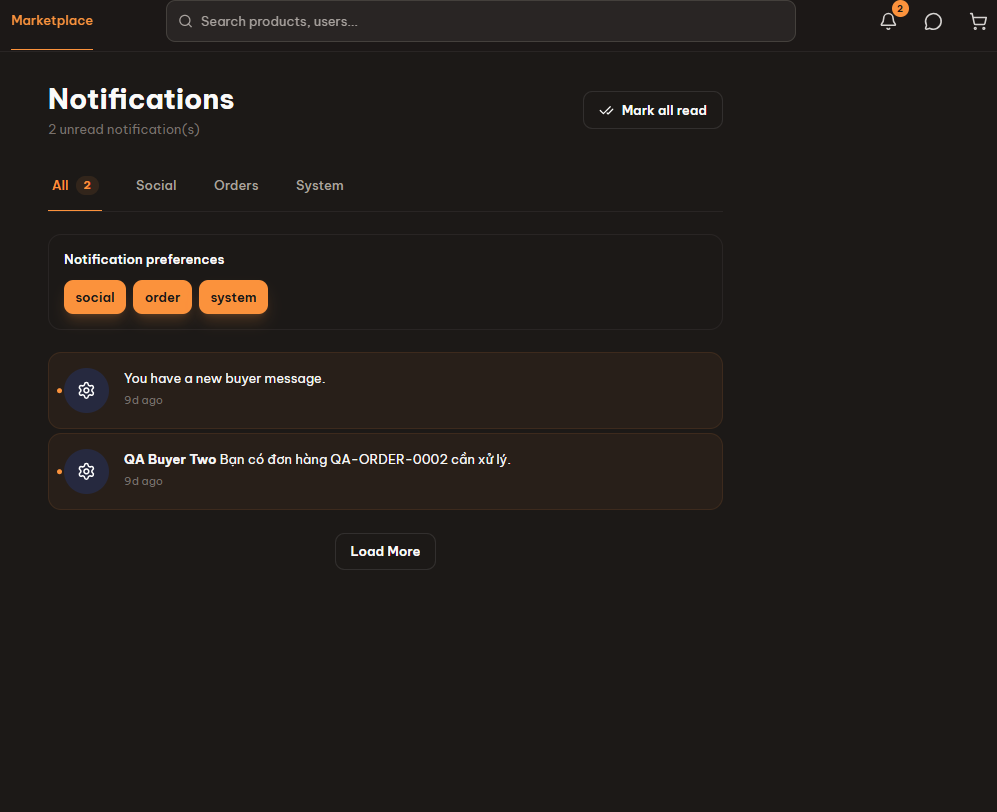
\includegraphics[width=\textwidth]{Images/UI/module7/notifications-page.png}
\caption{Giao diện trang thông báo}
\label{fig:module7-notifications-page}
\end{figure}

\subsubsection{Component Thông báo Real-time}

Hệ thống hỗ trợ thông báo real-time nhằm cập nhật nhanh các sự kiện mới như tin nhắn, tương tác bài viết hoặc cập nhật đơn hàng mà không cần tải lại trang. Các thông báo sẽ hiển thị dưới dạng popup trực tiếp trên giao diện người dùng nhằm đảm bảo trải nghiệm sử dụng liền mạch và thuận tiện hơn.

Người dùng có thể đóng nhanh thông báo hoặc truy cập trực tiếp đến nội dung liên quan từ popup thông báo real-time.

\begin{figure}[H]
\centering
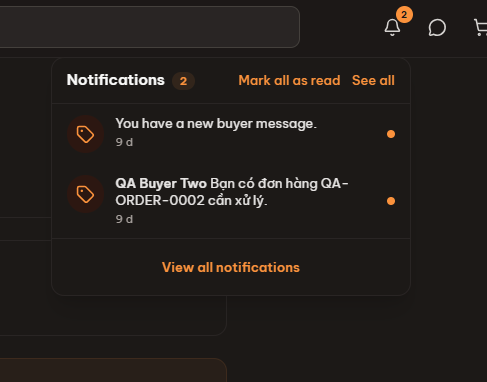
\includegraphics[width=0.6\textwidth]{Images/UI/module7/realtime-notification-popup.png}
\caption{Component thông báo real-time}
\label{fig:module7-realtime-notification-popup}
\end{figure}




